\documentclass[a4paper,11pt]{article}

%Les packages pour écrire des math
\usepackage{amsmath}
\usepackage{amsthm}
\usepackage{amssymb}
\usepackage{mathabx}
\usepackage{dsfont} %Fonction caractéristique
\usepackage{stmaryrd}
\numberwithin{equation}{section}

\usepackage{listings}
\usepackage[authoryear]{natbib}


\usepackage{hyperref}
\usepackage{url}

\usepackage{algorithm}
\usepackage{algorithmic}

%\usepackage[francais]{babel}	
\usepackage[utf8]{inputenc}
%\usepackage[T1]{fontenc}

\usepackage{graphicx}
%\usepackage{pst-solides3d}
\graphicspath{ {./images/} }
\usepackage[font=small,labelfont=bf]{caption}
\usepackage{subcaption}


\textwidth16cm
\oddsidemargin-0.55cm
\textheight22.5cm
\topmargin-2cm
\pagestyle{plain}
\setlength{\skip\footins}{1.2cm}


\renewcommand {\algorithmicrequire } {\textbf{\textsc{Entrée(s):} } }
\renewcommand {\algorithmicensure } {\textbf{\textsc{Sortie:} } }
\renewcommand {\algorithmicwhile } {\textbf{Tant que} }
\renewcommand {\algorithmicdo } {\textbf{faire} }
\renewcommand {\algorithmicendwhile } {\textbf{fin du Tant que} }
\renewcommand {\algorithmicif } {\textbf{Si} }
\renewcommand {\algorithmicfor } {\textbf{Pour} }
\renewcommand {\algorithmicendfor } {\textbf{fin du Pour} }
\renewcommand {\algorithmicthen } {\textbf{alors} }
\renewcommand {\algorithmicendif } {\textbf{fin du Si} }
\renewcommand {\algorithmicelse } {\textbf{Sinon} }
\renewcommand {\algorithmicreturn } {\textbf{Renvoyer} }

\newtheorem{theorem}{Théorème}[section]
\newtheorem{conjecture}{Conjecture}
\newtheorem{lemma}{Lemme}
\newtheorem{proposition}{Proposition}
\newtheorem{corollary}{Corollaire}
\newtheorem{definition}{Définition}
\newtheorem{example}{Exemple}
\newtheorem{note}{Note}



\begin{document}
	\begin{center}
			
\includegraphics[scale=0.5]{images/LSCE.jpg}
	\end{center}
	\hypersetup{pdfborder=0 0 0}
	\newcommand{\HRule}{\rule{\linewidth}{0.5mm}}
	\begin{center}
		\textsc{\LARGE Laboratoire des Sciences du Climat} \\[0.3cm]
		\textsc{\LARGE et de l'Environnement}\\[1.5cm] 
		\HRule \\[0.5cm]
		{\huge \bfseries Changement d’échelles dans les projections climatiques et leurs impacts hydrologiques: Cas des grandes plaines américaines}\\[0.4cm] 
		\HRule \\[1.5cm]
	\end{center}
	\begin{center}
	\begin{minipage}{0.4\textwidth}
		\begin{flushleft} \Large
			\emph{Auteur}\\
		\end{flushleft}
	\end{minipage}
	~
	\begin{minipage}{0.4\textwidth}
		\begin{flushright} \Large
			\emph{Maîtres de stage} \\
		\end{flushright}
	\end{minipage}\\[0.5 cm]
	\begin{minipage}{0.4\textwidth}
		\begin{flushleft} \large
			\textsc{Mathis Deronzier}\\
			\textsc{Mines Saint-Étienne}
		\end{flushleft}
	\end{minipage}
	~
	\begin{minipage}{0.4\textwidth}
		\begin{flushright} \large
			\textsc{Emmanuel Mouche}\\
			\textsc{C.E.A.}\\
			\textsc{Mathieu Vrac}\\
			\textsc{C.N.R.S.}
		\end{flushright}
	\end{minipage}\\[2cm]
	\end{center}
	\begin{center}
		\textsc{\Large Stage de recherche de master 2}\\[0.5cm]  
		\large Avril-Septembre\\2021\\[2cm]
	\end{center}

\newpage
\tableofcontents

\newpage
\section{Introduction}
\label{ch:introduction}

\subsection{Contextualisation et motivations du stage}
\label{ch:Contextualisation et motivations du stage}

Alors que le rapport du GIEC 2021 sorti cet été projette une augmentation de la température mondiale moyenne de $1.5^{\circ}$C d'ici $2050$ ainsi que des modifications des climats dans plusieurs régions du monde. Il semble aujourd'hui primordial de comprendre les conséquences locales d'un changement climatique global. Les changements climatiques locaux sont des enjeux politiques et économiques majeurs et leurs prévisions sont des problématiques centrales pour la population mondiale.

Les projections climatiques sont données par des modèles de climat travaillant à l'échelle de l'ordre d'une centaine de kilomètres, on cherche alors à prévoir des résultats sur des zones plus localisées. Le domaine du climat étudiant les questions de changement d'échelle du global au local est le \textit{downscaling}. La question inverse du changement d'échelle du local au global est non moins intéressante pour les climatologues. En effet, comment savoir si les modèles à grande échelle sont vraiment représentatifs de la réalité? Alors que les modèles climatiques et hydrologiques travaillent sur des échelles globales, les lois de la physique sont elles, locales. On cherche alors à comprendre à partir des équations de la physique les interactions ou équations qu'elles engendrent à grande échelle, ce domaine de recherche s'appelle l'\textit{upscaling}. 

C'est dans ces problématiques de changement d'échelle que s'ancre ce stage. Pour concentrer et enrichir nos réflexions, nous nous intéresserons plus précisément à la question de l'impact du changement d'échelle sur les modélisations hydrologiques. Afin de concrétiser ces problématiques, nous avons modélisé le fonctionnement hydrologique du bassin du Little Washita. 
Le domaine d'étude ayant été choisi pour modéliser et concrétiser ces problématiques a été le bassin du Little Washita. Ce bassin situé aux États-Unis dans l’état d’Oklahoma, possède de nombreuses caractéristiques qui le rendent intéressant. Sa superficie de $611km^2$ est de l'ordre de grandeur d'une maille de modèle continentale et il a déjà fait l'objet de nombreuses études (voir par exemple \cite{maxwell2007groundwater}, \cite{rosero2011ensemble}, \cite{maquin2016developpement}). 

\vspace{0.7cm}

Pour s'intéresser à la question du changement d'échelle il fallait pouvoir comparer des données à grande échelle et à petite échelle. Les données NARR (North American Regional Reanalysis\footnote{Les reanalysis sont des modèles de climats simulés que l'on force à prendre certaine valeurs mesurées pour certains points et certains temps, nous considérerons les données NARR comme les données climatiques réelles.}) allant de l'année $1979$ à $2014$ semblaient constituer un jeux de données pertinent pour l'étude du Little Washita. En effet, sa longueur de maille de $32km$ permettait à la fois de considérer l'upscaling hydrologique sur de ce bassin et le downscaling pour des jeux de données sur des échelles plus larges. Pour obtenir ces données à grande échelle nous avons opté pour deux types de données: les données l'IPSL qui possèdent une longueur de maille de $200km$ ainsi que les données NARR considérées à plusieurs échelles différente (ce point sera développé dans la section \ref{ch:proj-climatique-mod-hydro}). Ainsi, si les données IPSL et NARR sont peut-être décorrélées on est absolument certain que les données NARR et leurs dégradées le sont. L'objectif aura été dans un premier temps de regarder différentes méthodes de downscaling pour améliorer les projections des données NARR à partir des séries à plus grande échelle. Une fois cette étape effectuée, il s'agissait de réaliser une simulation hydraulique sur les années prédites et de comparer l'impact du downscaling sur les résultats des simulations hydrologiques. La problématique de l'upscaling sera en fait cachée dans la modélisation hydrologique du bassin du Little Washita, bien qu'elle n'ait pas été concrètement traitée dans les faits, elle a été centrale dans notre réflexion. Finalement, nous avons donné les conclusions que nous avons tirées dans.

\subsection{Présentation du plan}
\label{ch:presentation plan}

Dans la première partie nous allons introduire rigoureusement le concept de downscaling et les outils utilisés pour mesurer la qualité de nos prédictions. Nous verrons l'algorithme \textit{Cumulative Distribution Function transfert} (CDFt), celui utilisé pour downscaler nos séries. Nous introduirons le transport optimal généralisant l'algorithme CDFt. Nous verrons ensuite comment estimer la qualité de nos prédictions, puis nous étudierons les distances de Kolmogorov Smirnov et celle de Cramér-von Mises permettant de quantifier la différence entre deux lois. 

La seconde partie sera consacrée à la physique et la modélisation. Elle présentera les principaux mécanismes de la modélisation hydrologique ainsi que les modèles d'Orchidée et d'HydroGéoSphère. Dans un premier temps nous présenterons les interactions sol-atmosphère ainsi que les caractéristique des sols et leur influence sur les débits. Nous présenterons ensuite les principales équations de la mécanique des fluides en milieu poreux, puis deux modèles utilisés pour les modélisations hydrologiques, Orchidée et HydroGéoSphère en expliquant plus en détail la problématique de l'upscaling.

La troisième et dernière partie présentera la démarche, les résultats ainsi que les questionnements que nous avons eu à mesure de nos résultats. Nous commencerons par expliquer en détail la méthodologie que avons suivie, puis nous présenterons pas à pas les résultats obtenus.


\newpage
\section{Changement d'échelle, downscaling et analyse des résultats}
\label{ch:downscaling}
Cette section se concentre sur la partie statistique du stage, on cherchera à partir de données à grande échelle issues de modèles climatiques et de données réelles à améliorer les projections des variables de précipitation et d'évapotranspiration sur le bassin versant du Little Washita. 

Nous commencerons par formaliser rigoureusement le downscaling statistique, puis nous réintroduirons les concepts mathématiques essentiels à la compréhension de l'algorithme CDFt. Nous verrons ensuite comment nous pouvons généraliser le principe de l'algorithme CDFt avec la méthode du transport optimal. Pour terminer nous verrons les méthodes de test pour évaluer la qualité de prédictions sur plusieurs années.

\vspace{0.7cm}

Le downscaling statistique (voir par exemple \cite{vrac2012dynamical} et \cite{ayar2016intercomparison}) est une méthode utilisée dans les sciences du climat permettant d'améliorer les projections des modèles climatiques. À partir des données obtenues par un modèle de climat (modèle de circulation général, modèle climatique régional) et des données observées sur la zone que l'on cherche à prédire, on essaie de corriger les biais systématiques introduits par les modèles. Le nom ``downscaling'' vient du domaine d'application de cette méthode. On passe généralement d'un modèle à grande échelle à des données observées à petite échelle. Nous n'expliquerons que deux méthodes de downscaling mais d'autres méthodes existent, l'article de \cite{ayar2016intercomparison} donne un aperçu des différentes méthodes existantes.

\vspace{0.7cm}

Pour formuler rigoureusement l'approche du downscaling nous introduisons des hypothèses communément admises dans les sciences du climat. On suppose que les variables étudiées sont des variables aléatoires réelles dépendantes du temps et de l'espace, on appelle $\mathcal{M}(\Omega,\mathbb{R})$ l'espace des variables aléatoires réelles et $S(\mathbb{R}^3)$ la spère unité dans $\mathbb{R}^3$. On suppose de plus que l'on peut faire correspondre chaque point de la terre à un point de la sphère unité. Nous travaillerons par la suite sur la sphère unité que l'on considérera être la terre.

\begin{definition}
	\label{terre}
	Pour une variable quantitative $V$ à valeur dans $\mathbb{R}$, on appelle $\mathcal{T}_V$ la fonction donnant les  valeurs réelles de cette variable sur la terre à un moment donné, formellement (en considérant la terre comme une sphère $\mathcal{S}(\mathbb{R}^3)$) nous avons
	\begin{equation}
		\label{eq-terre-mod}
		\begin{array}{ccc}
			\mathcal{T}_V: \mathbb{R}_{+}\times\mathcal{S}(\mathbb{R}^{3}) & \to & \mathcal{M}(\Omega,\mathbb{R}).
		\end{array}
	\end{equation}
	Alors, $\mathcal{T}_V(t,x)$ est la valeur de la variable au temps $t$ au point de coordonnée $x$ sur terre.	
\end{definition}

\begin{definition}
	\label{simu_terre}
	On appelle simulateur de variable quantitative $V$ à valeur dans $\mathbb{R}$, une fonction $S_V$ satisfaisant:
	\begin{equation}
		\begin{array}{ccc}
			S_V: \mathbb{R}_{+}\times\mathcal{S}(\mathbb{R}^{3}) & \to & \mathcal{M}(\Omega,\mathbb{R}).
		\end{array}
	\end{equation}
\end{definition}
On peut alors estimer la qualité des simulations en mesurant une distance entre la réalisation $\mathcal{T}_V([0,T])$ et celle de $S_V([0,T])$. Le travail du downscaling est de trouver des transformations sur les variables aléatoires $S_V(t,x)$ pour minimiser ces distances. Plusieurs méthodes peuvent-être utilisées pour réduire ces distances. Une approche géostatistique  existe pour étudier ces problématiques. Par exemple, des méthodes de résolution d'équations différentielles permettent d'interpoler les résultats (voir par exemple \cite{lindgren2011explicit}), ce n'est pas cette axe que nous allons prendre dans ce stage mais plutôt celui des transformations sur les variables aléatoires à une autre.

\subsection{Introduction à la problématique du downscaling}
\label{ch:intro-dwnsc}
Le downscaling que nous étudions ici, consiste donc à considérer des transformations sur des variables aléatoires réelles. Pour étudier ces variables aléatoires et construire les transformations on commence par introduire ici les notions de \textbf{fonction de répartition}, \textbf{fonction de répartition empirique} ainsi que celle de \textbf{fonction de densité}. Ces notions sont centrales dans les méthodes de downscaling que nous allons expliquer.

\begin{definition}
	Soit $X$ une variable aléatoire réelle, on appelle \textbf{fonction de répartition de $X$}, $\mathcal{F}_{X}: \mathbb{R}\to [0,1]$ la fonction vérifiant
	\begin{equation}
		\mathcal{F}_{X}(x)=P(X\leq x).
	\end{equation}
\end{definition}

\begin{definition}
	Soient $X_1,X_2,...,X_n$, n réalisations indépendantes d'une variable aléatoire réelle $X$, on appelle \textbf{fonction de répartition empirique de $X$}, la fonction $\mathcal{F}_{n}:\mathbb{R}\to [0,1]$ définie par
	\begin{equation}
		\mathcal{F}_{n}(x)= \frac{1}{n}\sum_{i=1}^{n}\mathds{1}_{[X_i, +\infty )}(x).
	\end{equation}
\end{definition}

\begin{definition}
	Soit $X$une variable aléatoire réelle, on note $f_{X}$ la \textbf{fonction de densité de $X$}, $f_{X}: \mathbb{R}\to [0,\infty[$ la fonction vérifiant
	\begin{equation}
		f_{X}(x)=\lim_{t\to 0} \frac{P(x\leq X \leq x+t)}{t}.
	\end{equation}
\end{definition}
Remarquons qu'une variable aléatoire ne possède pas nécessairement de fonction de répartition (notamment les variables aléatoires à valeurs discrètes), on peut cependant les étudier dans la théorie des distributions \cite{golse2020distributions}.

Commençons par établir notre problématique dans le cas le plus simple où l'on cherche à projeter une variable $V$ dans l'avenir alors que nous connaissons ses réalisations dans le passé à un endroit donné $x$.
On peut alors considérer deux processus aléatoires à valeurs dans $\mathbb{R}$, 
\[(X_t)_{t \in \mathbb{N}}=(\mathcal{S}_{V}(t, x))_{t \in \mathbb{N}} \textrm{ et } (Y_t)_{t \in \mathbb{N}}=(\mathcal{T}_{V}(t, x))_{t \in \mathbb{N}}.\]

La problématique à laquelle nous cherchons de répondre est la suivante: connaissant $X_1,X_2,...,X_n$ et $Y_1,Y_2,...,Y_n$ les réalisations jusqu'au temps $n$ ainsi que $X_{i_1},X_{i_2},...,X_{i_m}$ (pour des temps futurs), on cherche une fonction $G: \mathbb{R} \to \mathbb{R}$ telle que les tirages $G(X_{i_1}),..., G(X_{i_m})$ et $Y_{i_1},...,Y_{i_m}$ soient proches du point de vu de leur loi (nous éclaircirons ce point dans la section \ref{analyse-pred}). 

Autrement dit, en appelant $X$ et $Y$ les réalisations de $(X_t)_{t \in \mathbb{N}}$ et $(Y_t)_{t \in \mathbb{N}}$ sur $\{1,...,n\}$ et $X'$ et $Y'$ les réalisations de $(X_t)_{t \in \mathbb{N}}$ et de $(Y_t)_{t \in \mathbb{N}}$ sur $\{i_1,...,i_m\}$, on cherche à définir $G_{X,Y}$ à partir de $X$, $Y$ tel que $G_{X,Y}$ minimise 
\[d(\mathcal{F}_{G_{X,Y}(X')}, \mathcal{F}_{Y'}),\]
où $d$ est une distance définie sur les fonctions.
Nous voulons aussi que $G_{X,Y}$ respecte certaines propriétés. Une des propriétés qui nous intéresse est celle de la consistance de notre transformation.

\begin{definition}
	Soient $X$ et $Y$ deux variables aléatoires réelles et $G_{X,Y}: \mathbb{R}\to \mathbb{R}$ une transformation, on dit que $G_{X,Y}$ est \textbf{consistante vis à vis de $X$ et de $Y$} si elle vérifie 
	\begin{equation}
		\label{cond-cons}
		{\mathcal{F}_{G_{X,Y}(X)}}= \mathcal{F}_{Y}.
	\end{equation}
\end{definition}
Dans la suite les transformations que nous considérerons satisferont toujours l'équation \eqref{cond-cons}.

\subsection{Cumulative Distribution Function transform (CDFt)}
\label{ch:CDFt}

Nous allons ici présenter l'algorithme principalement étudié et utilisé dans ce stage, l'algorithme CDFt (voir \cite{vrac2012dynamical}). Nous commencerons par présenter l'algorithme \textbf{quantile-quantile} permettant de comprendre l'esprit des transformations $G$ affectées aux processus aléatoires. Puis nous décrirons l'algorithme de CDFt-t. 

\subsubsection{Quantile-Quantile}
\label{Q-Q}
Le quantile-quantile consiste simplement à définir $G_{X,Y}$ la transformation permettant de passer de la fonction de distribution de $X$ à celle de $Y$. 
\begin{proposition}
	\label{prop:QQ_formula}
	Soit $X$ et $Y$ deux variables aléatoires réelles ayant des fonctions de répartition $\mathcal{F}_{X}$ et $\mathcal{F}_{Y}$ continues, alors 
	$\mathcal{F}^{-1}_Y (\mathcal{F}_X(X))$ et $Y$ suivent la même loi. 
\end{proposition}
On peut retrouver la démonstration de cette proposition dans les annexes section \ref{ch:outils-mathematiques}. Le principe de l'algorithme \textbf{quantile-quantile} est alors de calculr la transformation $G=\mathcal{F}^{-1}_{Y} \circ \mathcal{F}_{X}$. Ainsi, $\mathcal{F}_{G(X)}=\mathcal{F}_{Y}$ et l'on définit alors $G_{X,Y}=G$. L'une des limites de cette méthode est que le support de $f_{G(X)}$ est inclus dans celui de $f_{Y}$, alors les valeurs prises par $G_{X,Y}(X')$ seront incluses dans le support de $f_Y$. Nous aimerions alors que $X'$ ait aussi une influence sur le support des valeurs prises. Ce qui n'est pas le cas dans la transformation $G$ défini par la proposition \ref{prop:QQ_formula}. C'est en partie cette observation qui motive l'étude d'autres transformations. 

\subsubsection{CDFt}
\label{CDf-t-algo}

L'algorithme de \textbf{Cumulative Distribution Function transfer} (CDFt) vise à remédier au problème des bornes en appliquant des transformations sur les lois $X$ et $Y$. On considère les réalisations $X_1,..,X_n$ et $Y_1,...,Y_n$ ainsi que $X'_{1},...,X'{m}$.

\vspace{0.7cm}

\noindent \textbf{CDFt avec support égale}:

On peut par exemple faire en sorte que la transformation sur les projections conserve le support de celles-ci en d'autres mots on veut
\[ \min_{i \in I}(X'_i)=\min_{i \in I}(G_{X,Y}(X'_i)) \hspace{3mm} \textrm{et} \hspace{3mm}  \max_{i \in I}(X'_i)=\max_{i \in I}(G_{X,Y}(X'_i)).\]
Il suffit de transformer la loi de $Y$ sur $[0,1]$, de réaliser un quantile-quantile puis d'effectuer la transformation inverse. Concrêtement, nous posons 
\[\overset{\sim}{Y}= \frac{(Y-\min_{i\in I}Y_i)}{\max_{i\in I}Y_i- \min_{i\in I}Y_i}.\]
Alors, quelque soit $i$ dans $I$ on a $\overset{\sim}{Y}_i \in [0,1]$. En appelant $G= \mathcal{F}_{X,\overset{\sim}{Y}}$ la transformation quantile-quantile de $X$ à $\overset{\sim}{Y}$ on a $G_{X,Y}(X'_i) \in [0,1]$, la transformation s'imposant naturellement est alors
\[ G_{X,Y}= (\max_{i\in I}Y_i- \min_{i\in I}Y_i)G + \min_{i\in I}Y_i.\]
C'est l'une des premières idées lorsqu'on parle de transformations que l'on peut appliquer sur nos variables. Notons que l'on a aussi une grosse base de données et que l'on peut aussi essayer d'utiliser des méthodes de regression linéaire ou de machine learning pour estimer les max et les min de $Y'$ en fonction de $X$. Nous allons illustrer l'usage d'une de ces méthodes dans la prochaine partie \ref{CDFt reg l}.

\vspace{0.7cm}

\noindent \textbf{CDFt avec méthode de prédiction}
\label{CDFt reg l}

Supposons que l'on ait des fonctions estimant la variance et la moyenne de $Y'$ à partir de $X'$, s'exprimant sous la forme $\overline{f(X')} = \overline{Y'}$ ainsi que $\overline{g(X')} = \overline{\sigma(Y')}$ (on définit par $\overline{X}$ la  moyenne $X$ et par $\sigma(X)$ son écart type). Ces fonctions peuvent être obenues par des méthodes de régression linéaire sur des sous échantillons des données de $X$ et $Y$ soit après les avoir ordonnées si les $X_i$ et les $Y_i$ sont indépendants soit en fonction de leur indice.

On aimerait alors que $G_{X,Y}$ conserve la moyenne ainsi que la variance. Formellement, on voudrait définir $G_{X,Y}$ telle que quelque soient $\{i_1,...,i_m\}$ un ensemble d'entiers consécutifs et $X'$ et $Y'$ les vecteurs des variables aléatoires des $X_{i_j}$ et $Y_{i_j}$ sur cet ensembles, on ait :

\begin{equation}
	\label{cond-mu}
	\overline{G_{X,Y}(X')}=\overline{Y'},
\end{equation}
ainsi que
\begin{equation}
	\label{cond-sigma}
	\sigma({G_{X,Y}(X')})=\sigma(Y'),
\end{equation}
et que $G$ respecte la condition de consistance \eqref{cond-cons}.
Concrêtement, nous allons faire des transformations sur les variables aléatoires pour avoir ces conditions là. En appelant $G_{X,Y}= \mathcal{F}^{-1}_{Y}\circ\mathcal{F}_{X}$ on peut définir la transformation $G_{X,Y,X'}$

\[ G_{X,Y} (X')= \overline{g(X')}\frac{\mathcal{F}^{-1}_{Y}\circ\mathcal{F}_{X}(X')- \overline{\mathcal{F}^{-1}_{Y}\circ\mathcal{F}_{X}(X')}}{\sigma(\mathcal{F}^{-1}_{Y}\circ\mathcal{F}_{X}(X'))} + \overline{f(X')}.\]

On peut vérifier facilement que $G_{X,Y}$ ainsi défini respecte bien les propriétés \eqref{cond-cons} \eqref{cond-mu} et \eqref{cond-sigma}. L'idée est alors de trouver les fonctions $f$ et $g$ par des méthodes de regression linéaires. Remarquons aussi que lorsque la loi est bornée cela ajoute une condition supplémentaire à $G_{X,Y}$ et l'on ne peut pas nécessairement avoir les conditions sur la moyenne et la variance. Il faut alors choisir parmi l'une des conditions \eqref{cond-mu} et \eqref{cond-sigma}, c'est par exemple le cas pour les précipitations qui ne peuvent être négatives. 
\begin{note}
	Remarquons que l'efficacité des transformations que nous avons décrites repose en partie sur la stationnarité des lois suivies par les variables aléatoires aléatoires au cours du temps. Les questions de stationnarité ont été abordées dans \cite{maraun2012nonstationarities}, \cite{christensen2008need} ainsi que \cite{nahar2017assessing}. Il est notamment évident que la loi suivie par la température en été n'est pas la même que celle en hiver, et il en est de même pour toutes les autres variables climatiques.
\end{note}

Finalement, une des limites de l'algorithme de CDFt est dans le cas où plusieurs réalisations de $X'$ sont égales, elle seront renvoyées sur le même points. C'est vraiment problématique dans le cas où $X'$ possède plusieurs réalisations égales et que $\mathcal{F}_Y$ est une fonction continue (sans Dirac).

\begin{example}
	Soit $X$ une variable aléatoire qui possède comme probabilité 
	\[P(X=0)=\frac{1}{2} \textrm{ et } P( \frac{1}{2}\leq a\leq X \leq b\leq 1 )=b-a.\]
	et $Y$ une variable aléatoire réelle suivant la loi uniforme sur $[0,1]$. Pour transormer $X$ en $Y$ on aimerait que pour chaque $i\in \{1,...,n\}$ tel que $X_i=0$, $G(X_i)$ suivent une loi uniforme sur $[0,1/2]$ ce qui n'est pas possible avec les transformations que nous avons considérées.
\end{example}  
C'est en partie à ce problème que répond le transport optimal.

\subsection{Transport optimal}
\label{ch:transport-optimal}

Nous voulons à la fois projeter la précipitation et l'évapotranspiration, on peut alors considérer une seule variable aléatoire dans $\mathbb{R}^2$. On peut généraliser l'idée utilisée précédemment pour trouver une méthode permettant de corriger les biais statistiques introduits par les modèles de projection. Cette méthode a d'autant plus d'intérêt que la variable utile dans les modèles hydrologique est 
\begin{equation}
	\label{eq-Qin-pr-etp}
	\textit{quantité d'eau entrant dans le sol}=\textit{précipitation}-\textit{évapotranspiration}.
\end{equation}
Comme l'objectif final est de projeter des résultats hydrologiques sur le bassin du Little Washita, il semble particulièrement pertinent de considérer la loi conjointe (précipitation, évapotranspiration\footnote{Nous utiliserons en réalité l'évaporation potentielle et nous verrons dans la section \ref{ch:generalite interaction atmosphere-surface continentale-sol} qu'il faut encore travailler pour obtenir l'évaporation finale.}). La théorie généralisant cette idée est la théorie du \textbf{transport optimal}.

La problématique du transport optimal a premièrement été introduite en par Gaspard Monge en 1781 puis a été développée par Kantorovitch en $1971$ et ses travaux pour l'allocution des ressources lui ont valu un prix nobel d'économie en $1975$. La formulation que nous en donnons par la suite est issue de \cite{villani2003topics}.

\subsubsection{Problématique}
\label{ch:s-Problematique}

Précédemment nous avons cherché à définir une transformation $G$ de la variable aléatoire $X$ telle $G(X)$ suive la même loi que $Y$. En considérant les fonctions de densité de $X$ et de $Y$ on a cherché à ce que la fonction de densité de $G(X)$ soit la même que celle de $Y$. On peut considérer une fonction de densité comme une mesure sur l'espace sur lequel on travail on a alors transformé une mesure $f_X$ en une autre mesure $f_Y$. Comme ces deux mesures sont de mesure totale égale à $1$, on peut dire que d'une certaine manière chaque ``poids'' de la mesure $f_X$ a été déplacé vers un ``poids'' de la mesure $f_Y$. L'idée du transport optimal est de trouver les déplacements naturels des poids d'une fonction de densité à une autre.  

Nous présenterons ici la formulation établie par Kantorovitch dans les années $70$ qui a l'avantage d'inclure celle de Monge.

Considérons deux fonctions de répartitions pour des variables aléatoires $U$ et $V$ à valeurs dans $A$ et $B$, on appelle ces fonctions $\mathcal{F}$ et $\mathcal{G}$ et on appelle $f$ et $g$ leurs fonctions de densités. On cherche alors une mesure $\pi$ sur  $A \times B$ satisfaisant
\[\int_{B} d\pi(x,y)= f(x), \hspace{4mm} \int_{A}  d \pi(x,y)= g(y),\]
de plus on veut que $\pi$ satisfaisant l'équation précédente minimise la quantité
\[\mathcal{I}[\pi]=\int_{A \times B}d(x,y) \, d\pi(x,y),\]
où $d$ est une certaine distance définissant le coût de transport de $x$ à $y$. Dans notre cas $U$ et $V$ sont des variables aléatoires à valeurs dans $\mathbb{R}^2$. Nous voyons que le choix de la distance a une influence majeure sur la mesure obtenue. On peut interpréter $d\pi(x,y)$ comme la quantité déplacée de $x$ à $y$.
\subsubsection{Résolution du problème dans le cas fini et downscaling}
La résolution de ce problème dans le cas fini a été traité de nombreuses fois. On utilisera les idées développées dans le papier \cite{robin2019multivariate}. Appelons $\pi \in \mathbb{R}^{m\times n}$ une matrice de transfert de poids dans le cas fini. On a $X_1,...,X_n$ ainsi que $Y_1,...,Y_m$ des réalisations de $X$ et de $Y$ et on cherche alors une matrice $\pi$ telle que 
\[\sum_{j=1}^{n} \pi_{i,j}= P(X=X_i) \textrm{ et } \sum_{i=1}^{m} \pi_{i,j}= P(Y=Y_j),\]
avec $\pi$ minimisant 
\[\mathcal{I}[\pi]=\sum_{i,j}d(X_i,Y_j)\pi_{i,j}.\]  
Le papier \cite{robin2019multivariate} utilise la norme euclidienne comme distance, l'obtention de cette solution peut se faire par un algorithme de simplexe, voir par exemple \cite{huang2012optimal}. Pour corriger le biais d'estimation on peut alors pour chaque $x$ tirés récupérer (par méthode de krigeage par exemple) le $\pi(x,\cdot)$. D'après la construction de $\pi$, on peut alors normaliser la fonction $y\mapsto \pi(x,y)$ et tirer aléatoirement un point selon la loi ainsi trouvée (voir \cite{robin2019multivariate} pour plus de détails). Nous n'avons pas utilisé cette méthode, bien qu'il aurait été très intéressant de voir ses résultats.


\subsection{Analyse des résultats obtenus par downscaling}
\label{analyse-pred}

L'analyse de nos résultats se fera par validation croisée, nous allons apprendre sur $50\%$ de nos données et faire nos projections sur les $50\%$ restants. La question à laquelle nous allons répondre dans cette partie est la suivante:

Comment évaluer la qualité de nos prédictions alors que nous avons réalisé des prédictions sur plusieurs années?

Contrairement à la manière habituelle de faire, consistant à estimer une distance entre chaque point projeté (souvent RMSE), en climatologie nous cherchons à comprendre la tendance générale. En effet, le paradigme d'évaluation en prévisions climatiques sur plusieurs années n'a pas l'ambition de prédire ponctuellement chaque prévision, mais il a pour objectif de décrire une tendance générale. On s'intéresse alors à des informations plus générales, c'est à dire que l'on travaille sur les lois de répartitions. Il faut alors réfléchir à des normes ou des distance pour évaluer la qualité de nos projections.  

\vspace{0.7cm}

Dans notre cas nous faisons des tests non-paramétriques, c'est à dire que l'on ignore tout des lois que nous comparons.
Différentes méthodes pour tester l'égalité de lois sont connues, nous n'en développerons que deux. Le mémoire \cite{ethier2011propos} donne une présentations de principaux tests statistiques permettant d'évaluer si oui ou non à partir des réalisations $X_1,...,X_n$, $Y_1,...,Y_n$ de deux lois inconnues sont les mêmes. 

Nous posons habituellement en statistiques deux hypothèses:
\[ \mathcal{H}_0: \mathcal{F}_{X} = \mathcal{F}_{Y} \hspace{3mm} et \hspace{3mm} \mathcal{H}_1: \mathcal{F}_{X} \neq \mathcal{F}_{Y},\]
où les égalités sur les lois sont en norme $L^p$. On suppose $\mathcal{H}_0$ et on définit une statistique sur $\|\mathcal{F}_{X}-\mathcal{F}_{Y}\|_{L^p(\mathbb{R})}$ permettant à partir de nos observations d'accepter ou de rejeter l'hypothèse $\mathcal{H}_0$.
Les tests de Kolmogorov-Smirnov et Cramer-von Mises utilisent à-peu-près cette idée. 


\subsubsection{Distance de Kolmogorov-Smirnov}
\label{ch:Kolmogorov-Smirnov-distance}
Le test d'ajustement  de  Kolmogorov-Smirnov \cite{buning2002robustness} est  l'un des plus  utilisé pour tester l'égalité de deux lois  de probabilités. Dans  le  contexte de  l'égalité de lois  de probabilité, la statistique  de  test  est 
\[K_{n,m}= \sqrt{\frac{nm}{n+m}}\|\mathcal{F}-\mathcal{F}_n\|_{\infty}.\]
La suite de variables aléatoires $K_{n,m}$ converge vers une variable aléatoire $K$ dont la fonction de survie est donnée par: 
\begin{equation}
	Q(x)=P(K>x)=\sum_{j=1}^{\infty}(-1)^{j-1}\exp(-2(jx)^2)
\end{equation}
On peut alors l'approximer avec les premiers termes de la série pour construire le test statistique. La démonstration de ce théorème peut être trouvée dans le livre \cite{walker1965probability}(chap 12.5). Nous voyons cependant que ce test est sensible aux données aberrantes, nous privilégierons alors le test de \textbf{Cramér-von Mises} \cite{buning2002robustness} (section \ref{ch:Cv-M distance}).


\subsubsection{Distance de Cramér-von Mises}
\label{ch:Cv-M distance}
On considère ici les deux fonctions de répartitions $\mathcal{F}_{n}$ et $\mathcal{G}_{m}$ continues des variables aléatoires $X$ et $Y$. Nous voulons tester les hypothèses
\begin{equation*}
	\mathcal{H}_0 : \mathcal{F}_{n} = \mathcal{G}_{m} \hspace{3mm}\textrm{et}\hspace{3mm} \mathcal{H}_1 : \mathcal{F}_{n} \neq \mathcal{G}_{m}.
\end{equation*}
Dans les tests proposés les statistiques sont construites à partir de deux échantillons indépendants des tests dans les cas où les variables $X$ et $Y$ sont indépendantes peuvent être trouvés dans \cite{ethier2011propos}. On définit aussi la fonction de répartition empirique $\mathcal{F}_n$.

Nous avons donc $n$ réalisations de $X$ et $m$ réalisations de $Y$ de lois de répartitions $\mathcal{F}$ et $\mathcal{G}$.
La statistique du test est définie par
\begin{equation}
	C_{n,m}=\frac{nm}{n+m}\int_{\mathbb{R}}\big[ \mathcal{F}_{n}(x)-\mathcal{G}_{m}(x)\big]^{2} \mathrm{d} \mathcal{H}_{m,n}(x),
\end{equation}
avec
\begin{equation}
	\mathcal{H}_{n,m}=\frac{n}{n+m}\mathcal{F}_n+\frac{m}{n+m}\mathcal{G}_m.
\end{equation}
$\mathcal{H}_{n,m}$ est alors la fonctions de répartitions empirique d'une variable aléatoire $Z$ construite à partir des $n+m$ réalisations indépendantes $X_1,...,X_n,Y_1,...,Y_m$. On peut simplement réécrire la valeur $C_{n,m}$
\begin{equation}
	C_{n,m}=\frac{mn}{(m+n)^2}\sum_{i=1}^{m+n}\big(\mathcal{F}_n(Z_i)-\mathcal{G}_{m}(Z_i)\big)^2.
\end{equation}

\begin{lemma}
	\label{C-v}
	On peut simplifier cette formule en supposant que les $(X_i)_{i\in \{1,...,n\}}$ et $(Y_i)_{i\in \{1,...,m\}}$ sont triés on a:
	\begin{equation}
		C_{n,m}=\frac{1}{nm(m+n)}\Big[ n\sum_{i=1}^{n}(R_{X_i}-i)^2+ m\sum_{i=1}^{m}(R_{Y_i}-i)^2\Big]-\frac{4nm-1}{6(m+n)}.
	\end{equation}
	où $R_{X_i}$ est le rang de $X_i$ dans $X_1,...,X_n,Y_1,...,Y_n$ autrement dit 
	\[R_{Z_i}=Card(\{z\in Z, z\leq Z_i\}).\] 
\end{lemma}
Ce lemme permet de simplifier algorithmiquement le calcul de cette intégrale.
\begin{note}
	La démonstration de cette formule se trouve dans l'indexe \ref{C-v} et la formulation de cette égalité diffère de celle contenue dans le mémoire \cite{ethier2011propos}(sec 2.3.2) qui contient une erreur.
\end{note}
Cette formulation a le bon goût de nous indiquer que la statistique ne dépend pas de la loi. On peut alors calculr simplement sa statistique sous l'hypothèse $\mathcal{H}_0$ pour la loi uniforme sur $[0,1]$ et ainsi retrouver les quantiles présentés dans l'article de \cite{buning2002robustness}. Nous voyons que l'idée du test est aussi de pondérer la différence des fonctions de répartition empiriques par les observations (l'intégration selon $\mathcal{H}_{m,n}$). Ainsi, si le test de Kolmogorov-Smirnov est sensible aux outliers, celui-ci l’est beaucoup moins lorsque les échantillons sont suffisamment grands. Malheureusement, dans la pratique les résultats renvoient quasiment toujours que les lois ne sont pas les mêmes, nous allons tout de même considérer cette distance qui nous l'avons vu possède une interprétation statistique.  

\newpage
\section{Présentation des modèles de climat et hydrologiques}
\label{ch:presentation modele climat}

Cette section se concentre sur la partie physique du stage, nous développerons les concepts clés à la compréhension des modèles hydrologiques donnerons un aperçu du fonctionnement des modèles climatiques en générale. 

\vspace{0.7cm}

Nous commencerons par contextualiser l'étude hydrologique dans les modèles de climat en présentant brièvement les interactions entre ces différents modèles. Nous introduirons ensuite les principaux phénomènes physiques intervenant dans l'étude hydrologique d'un bassin. Nous irons ensuite plus dans les détails des équations de Navier-Stokes et développerons la construction des principales équations de la mécanique des fluides en milieu poreux. Et pour finir nous présenterons deux modèles continentaux de simulation hydrologique très différents dans leur approche et essaierons de faire comprendre au lecteur les enjeux de l'upscaling dans la comparaison de ces deux modèles.

\subsection{Présentation d'un modèle de climat}
\label{modeles de climat/ concepts hydro}

``\textit{Un modèle climatique simule les interactions entre l'atmosphère, l'océan et les surfaces continentales. Grâce au modèle, les scientifiques ont des représentations numériques de la répartition géographique de différents paramètres, tels que la répartition des vents, des nuages, des masses d'eau...}'' Jean Louis Dufresne.

Les modèles interagissent entre eux selon un grand nombre d'équations mathématiques, et le maillage de simulation est alors un maillage multidimensionnel (figure \ref{fig-maillage multidimentionnel terre}). 

\begin{figure}[H]
	\begin{center}
		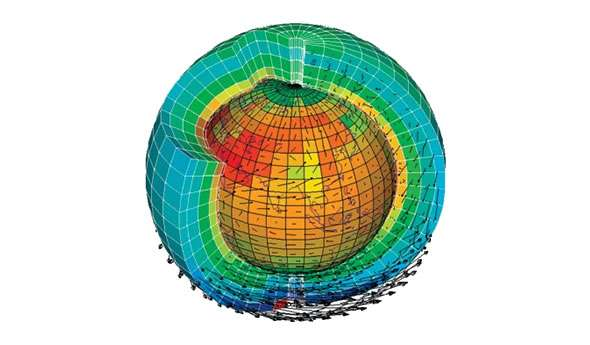
\includegraphics[scale=0.4]{maillage_terre.jpg}
	\end{center}
	\captionof{figure}{illustration d'un maillage multidimensionnel pour les modèles de climat}
	\label{fig-maillage multidimentionnel terre}
\end{figure}

La complexité des interactions entre les différents noeuds peuvent rendre les calculs vraiment laborieux. D'où l'intérêt de diminuer le nombre de mailles en passant à grande échelle puis downscaler les résultats obtenus. Nous présenterons dans la figure \ref{fig-modele de climat} les différentes interactions prises en compte dans l'élaboration du modèle de climat de l'IPSL.

\begin{figure}[H]
	\begin{center}
		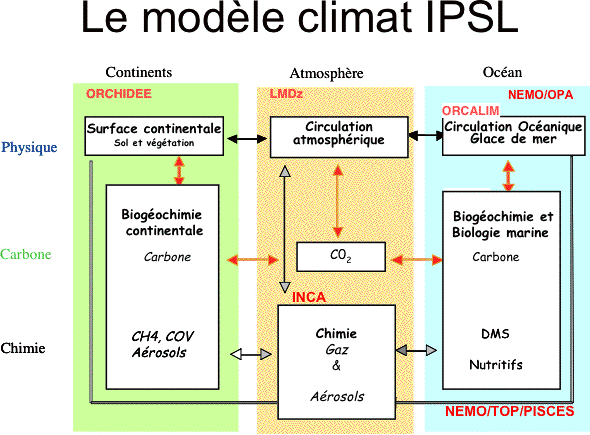
\includegraphics[scale=0.6]{modele_climat_IPSL.png}
	\end{center}
	\captionof{figure}{Présentation sommaire des différentes interactions dans le modèle de climat IPSL}
	\label{fig-modele de climat}
\end{figure}
	
Dans notre stage, nous nous sommes concentrés sur les modélisations continentales, à savoir, sur les interactions entre les modèles d'atmosphères et modèles continentaux ainsi que les mécanismes d'écoulement de l'eau dans les sols et les rivières. 

\subsection{Généralités sur les interactions atmosphère - surface continentale - sol}
\label{ch:generalite interaction atmosphere-surface continentale-sol}
Nous allons présenter ici les principales interactions entre la surface continentale et l'atmosphère. Cette étude a seulement pour objectif de donner un aperçu des différentes problématiques rencontrées dans l'élaboration des modèles continentaux. En effet, nous n'avons pas eu à nous soucier de toutes ces interactions dans l'étude que nous avons menée (section \ref{ch:proj-climatique-mod-hydro}) puisque les deux variables que nous avons utilisées étaient la précipitation et l'évapotranspiration potentielle: la première indiquant la quantité d'eau entrant dans le sol et la seconde la quantité d'eau sortant. Le plan de cette sous-section s'inspire très largement de la thèse \cite{maquin2016developpement}[chap 1] qui fournit d'avantage de détails et traite de la modélisation de l'ensemble des interactions dont nous allons parler.

\subsubsection{Les précipitations}
\label{ch:precipitations}

Ici, nous allons majoritairement utiliser les explications de la page internet cours EPFL sur les précipitations pouvant être trouvé \href{https://echo2.epfl.ch/e-drologie/chapitres/chapitre3/chapitre3.html}{\underline{ici}}, nous avons reformulé certaines parties et enlevé des détails mais la majorité de ce qui est écrit dans ce qui va suivre vient de cette page internet.
 
Sont dénommées précipitations, toutes les eaux tombant sur la surface de la terre, tant sous forme liquide (bruine, pluie, averse) que sous forme solide (neige, grésil, grêle) et les précipitations déposées ou occultes (rosée, gelée blanche, givre,...). Elles sont provoquées par un changement de température ou de pression. Les précipitations constituent l'unique ``entrée'' des principaux systèmes hydrologiques continentaux que sont les bassins versants. 

La formation des précipitations nécessite la condensation de la vapeur d'eau atmosphérique. La saturation est une condition essentielle à tout déclenchement de la condensation. Divers processus thermodynamiques sont susceptibles de réaliser la saturation des particules atmosphériques initialement non saturées et provoquer leur condensation:

\begin{itemize}
	\item Saturation et condensation par refroidissement isobare (pression constante),
	\item saturation et condensation par détente adiabatique (changement de pression sans échange de chaleur),
	\item saturation et condensation par apport de vapeur d'eau,
	\item saturation par mélange et par turbulence.
\end{itemize}
La saturation n'est cependant pas une condition suffisante à la condensation, cette dernière requiert également la présence de noyaux de condensation (impuretés en suspension dans l'atmosphère d'origines variées). Selon ces différents type de condensations les nuages crées et ainsi les précipitations varient.

\vspace{0.7cm}

\noindent \textbf{Types de précipitations}

\begin{itemize}
	\item Les précipitations convectives. Elles résultent d'une ascension rapide des masses d'air dans l'atmosphère. Elles sont associées aux cumulus et cumulo-nimbus, à développement vertical important. Les précipitations résultantes de ce processus sont en général orageuses, de courte durée (moins d'une heure), de forte intensité et de faible extension spatiale.
	\item Les précipitations orographiques. Comme son nom l'indique (du grec oros, montagne), ce type de précipitations résulte de la rencontre entre une masse d'air chaude et humide et une barrière topographique particulière. Par conséquent, ce type de précipitations n’est pas ``spatialement mobile'' et se produit souvent au niveau des massifs montagneux. Les caractéristiques des précipitations orographiques dépendent de l'altitude, de la pente et de son orientation, mais aussi de la distance séparant l'origine de la masse d'air chaud du lieu de soulèvement. En général, elles présentent une intensité et une fréquence assez régulières.
	\item Les précipitations frontales ou de type cyclonique. Elles sont associées aux surfaces de contact entre deux masses d'air de température, de gradient thermique vertical, d'humidité et de vitesse de déplacement différents, que l'on nomme ``fronts''. Les fronts froids (une masse d’air froide pénètre dans une région chaude) créent des précipitations brèves, peu étendues et intenses. Du fait d’une faible pente du front, les fronts chauds (une masse d’air chaude pénètre dans une région occupée par une masse d’air plus froide) génèrent des précipitations longues, étendues, mais peu intenses.
\end{itemize}

\subsubsection{Les écoulements}
\label{ch:ecoulement}

Les processus hydrologiques sont classiquement étudiés à l’échelle du bassin versant\footnote{Un bassin versant comme il est défini en hydrologie possède son équivalent en mathématiques, soit $(E,d)$ un espace métrique et $S:E\to E$ un endomorphisme sur $E$. On définit le bassin d'attraction d'un point $a$ qu'on appelle $B(a)$ l'ensemble des points $x$ dans $E$ tels que la suite $(x_n)_{n \in \mathbb{N}}=(S^n(x))_{n \in \mathbb{N}}$ converge vers $a$. En considérant qu'il existe une fonction $S$ définissant la trajectoire d'une goutte d'eau déposée au point $x$ les deux définitions ont la même signification en considérant le plus grand bassin d'attraction contenant un point $x$ choisi.}. En hydrologie, le bassin versant est une unité géographique définie par les limites topographiques que sont les lignes de crête. L’ensemble des écoulements converge vers les dépressions, formant ainsi un réseau hydrographique qui se dirige vers le point bas du bassin versant, l’exutoire. la figure \ref{fig-Bassin versant} définit un bassin versant. 

\begin{figure}[H]
	\begin{center}
		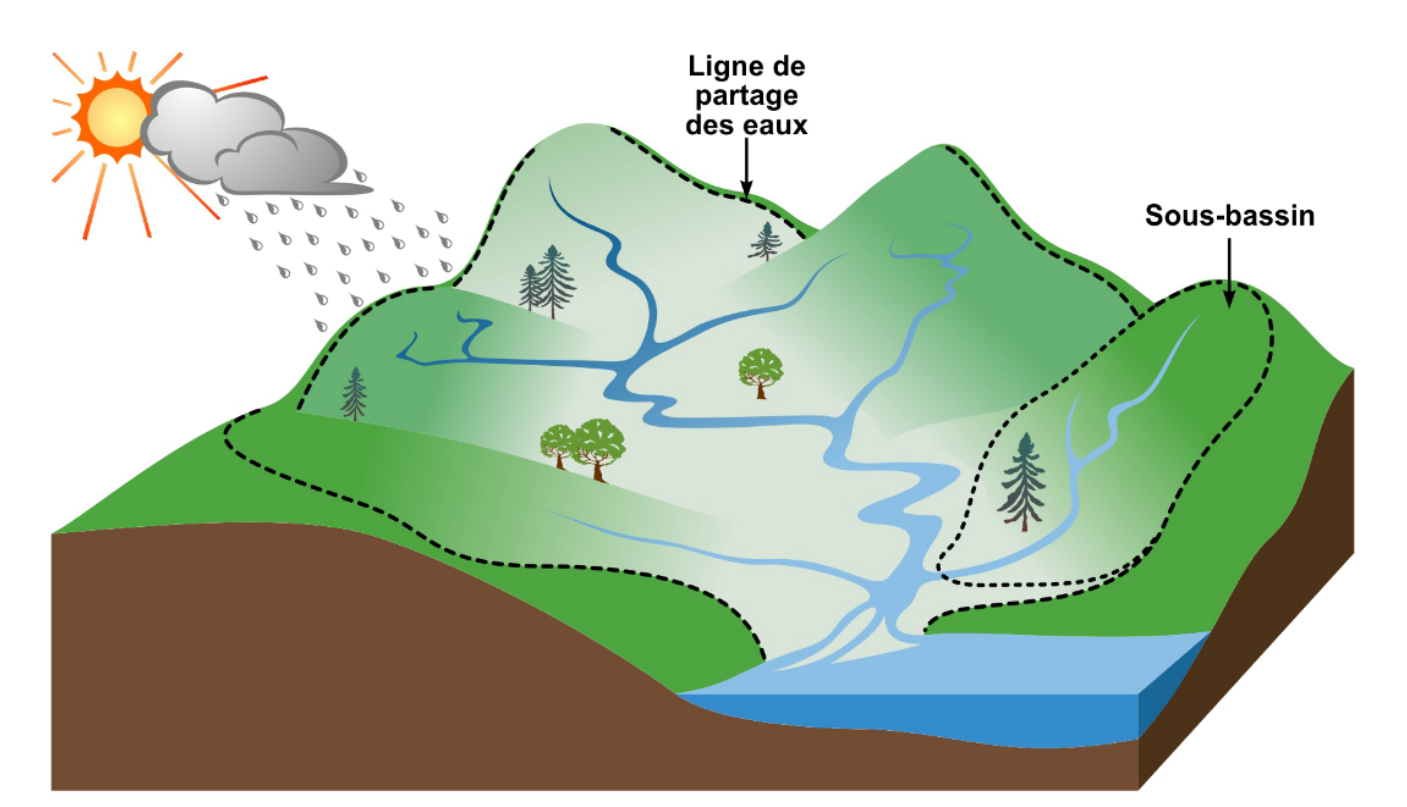
\includegraphics[scale=0.15]{bassin_versant.png}
	\end{center}
	\captionof{figure}{Bassin versant (Source :http://rqes-gries.ca/).}
	\label{fig-Bassin versant}
\end{figure}

À l’échelle du bassin versant, on distingue deux types d’écoulements: les écoulements de subsurface, les écoulements de surface. Les premiers sont des écoulements ayant lieux dans les pores du sols dans la région non saturée en eau (voir def \ref{def:saturation}) et les seconds en surface.


\vspace{0.7cm}

\noindent\textbf{Les écoulements de subsurface}:

La notion d'écoulement de subsurface se rapporte à l'écoulement de l'eau dans les pores du sol. Il dépend de plusieurs paramètres comme les caractéristiques du sol (sa porosité, sa perméabilité) c'est à dire la capacité qu'a l'eau à s'infiltrer dans le sol ainsi que la saturation en eau du sol, la topographie et le climat (précipitation, évaporation, transpiration). Ces écoulements sont traités par les équations de la mécanique des fluides (voir section  \ref{eq-Richards}), pour plus de détails se référer à \cite{maquin2016developpement} et \cite{marsily_de1986quantitative}. 

\vspace{0.7cm}

\noindent\textbf{Les écoulements de surface:}

Les écoulements de surface, aussi qualifiés de ruissellement, apparaissent lorsque le sol est saturé en surface et que le débit d'eau sur le sol est supérieur à sa capacité d'infiltration. Deux phénomènes distincts sont responsables du ruissellement, lorsque le sol est saturé, l’eau ne peut plus s’y infiltrer (voir \cite{cappus1960etude}). Cette condition de saturation à la surface du sol peut être la conséquence d'une nappe affleurant la surface, la zone satisfaisant cette propriété est appelée zone de suintement. Cela arrive aussi naturellement lors d'épisode pluvieux pour les nappes peu profondes. Le ruissellement peut aussi être causé par de fortes précipitations, ainsi le débit surfacique peut devenir supérieur à la quantité d'infiltration et ainsi créer un ruissellement. La quantité d'infiltration décroit exponentiellement lors d'évènements pluvieux (voir \cite{horton1933role}).  

\begin{center}
	\captionsetup{type=figure}
	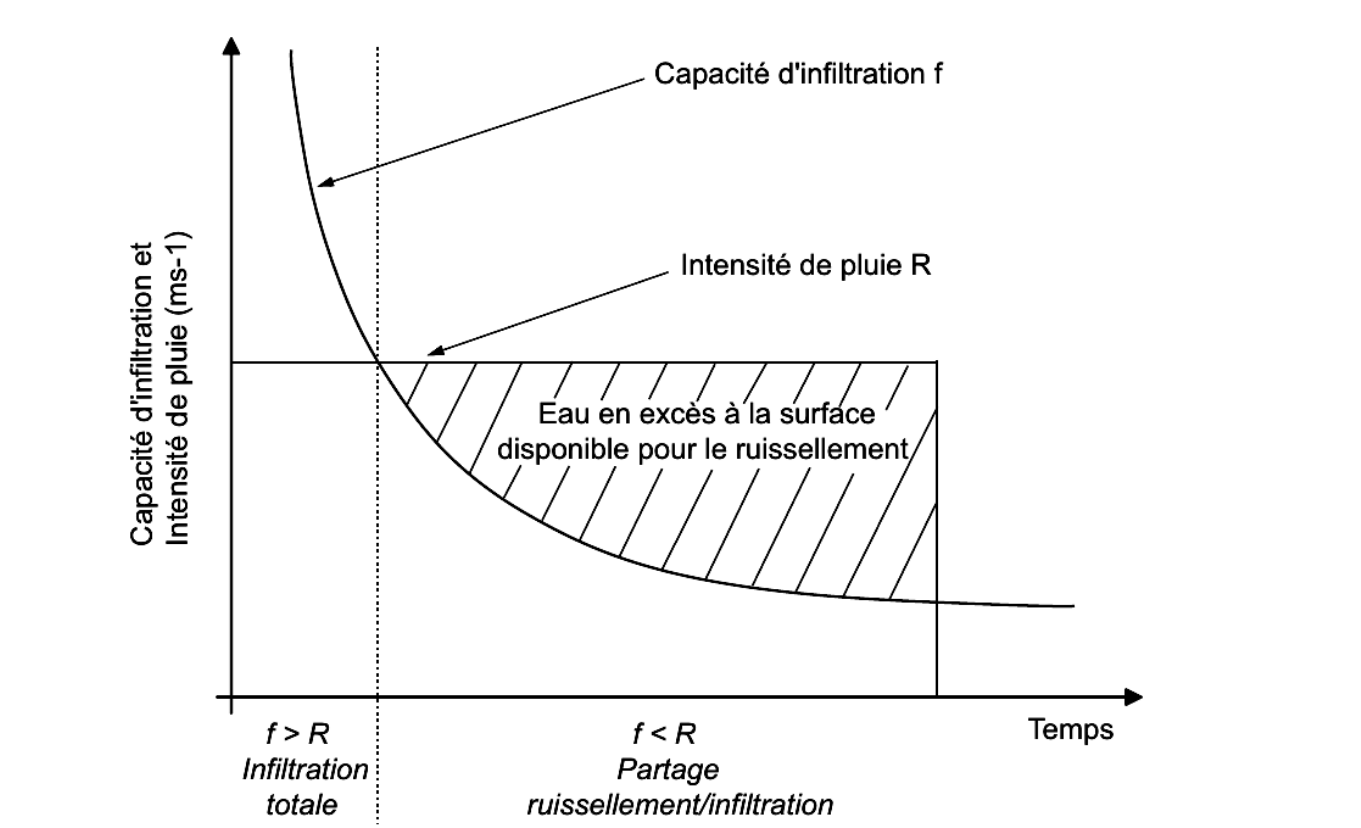
\includegraphics[scale=0.2]{ruissellement.png}
	\captionof{figure}{Estimation du ruissellement en fonction du temps, modèle de Horton (\cite{maquin2016developpement})}
\end{center} 

\vspace{0.7cm}

\noindent\textbf{Les interactions nappe rivière:}

Selon la position de la rivière par rapport à la nappe soit la nappe nourrit la rivière, soit c'est l'inverse, la figure \ref{fig-nappe_riviere} présente ce mécanisme.

\begin{figure}[H]
	\begin{center}
		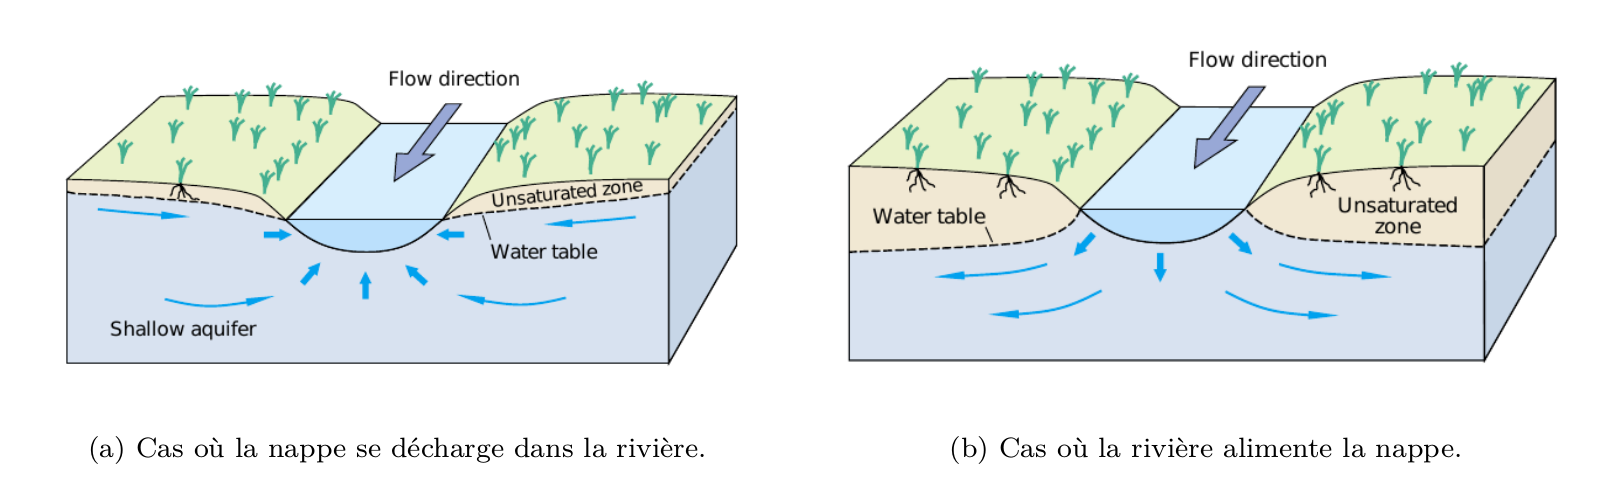
\includegraphics[scale=0.28]{nappe_riviere.png}
	\end{center}
	\captionof{figure}{Différente interactions entre la nappe et la rivière (thèse \cite{maquin2016developpement})}
	\label{fig-nappe_riviere}
\end{figure}

\subsubsection{Transferts d'eau entre le sol et l'atmosphère}
\label{ch:mecanismes}

La végétation constitue le lien entre l'atmosphère et le sol. Les végétaux sont les principales voies de transfert entre le sol et l'atmosphère, via les racines et la canopée. Il y a aussi des interactions directes entre la couche de surface du sol et l'atmosphère. Les trois principaux processus décrits sont: l'évaporation du sol, la transpiration des végétaux ainsi que l'évaporation de l'eau interceptée par la canopée. L'influence de la végétation a un très gros impact sur les modélisations hydrologiques, puisqu'elle influencent directement les flux d'eau dans le sol. 

\vspace{0.7cm}

\noindent\textbf{la transpiration:}

La ``transpiration'' des plantes consiste en une libération de vapeur d’eau par les plantes dans l’atmosphère. Ce phénomène constitue une réponse passive à l’environnement atmosphérique dû à l’existence d’un gradient de pression positif de l’atmosphère à la canopée, on parle aussi de demande atmosphérique. L’évaporation de l’eau par les plantes se produit dans les stomates des feuilles, de petites ouvertures où s’effectuent les échanges gazeux entre l’intérieur et l’extérieur de la plante. L’ouverture des stomates peut varier, régulant ainsi le flux de transpiration. Cette variation dans l’ouverture et la fermeture des stomates dépend de différents paramètres comme l’état hydrique du végétal ou les conditions climatiques.

La transpiration amène l'eau du sol par les racines puis les stomates vers l'atmosphère. La quantité d'eau transpirée dépend aussi du volume du sol couvert par les racine ainsi que de la teneur en eau du sol. Il arrive souvent en été, dans les régions arides, que la densité d'eau dans le sol ne soit pas suffisante pour qu'il y ait transpiration.

\vspace{0.7cm}

\noindent\textbf{Évaporation:}

Sur les surfaces de sol non recouvertes de végétation (sol nu), l’eau présente dans le sol, à proximité de la surface, peut s’évaporer. Ce phénomène apparaît en présence d’un gradient de pression de vapeur d’eau entre le sol et l’atmosphère et d’un apport d’énergie. L’évaporation effective dépend de l’état hydrique de la surface du sol, l’énergie pour extraire l’eau du sol augmentant à mesure que le sol s’assèche et des propriétés conductrices du sol (voir \cite{hillel2003introduction}).

\vspace{0.7cm}

\noindent\textbf{Pertes par interception:}

Lors d’un épisode pluvieux, une partie de l’eau incidente est interceptée par le feuillage. Il s’agit du phénomène dit d’interception. Cette eau, présente sur la canopée, peut ensuite s’évaporer directement. On désigne ce processus d’évaporation sur la canopée comme les pertes par interception. L’importance de ce flux d’eau dépend de l’ampleur du feuillage et de la capacité de stockage d’eau de la canopée, c’est-à-dire de l’épaisseur maximale de la lame d’eau par unité de surface de feuillage.

\vspace{0.7cm}

\noindent\textbf{L'évapotranspiration potentielle:}

On désigne par  ``évapotranspiration potentielle'' la quantité d’eau maximale que l’atmosphère peut extraire via les trois processus décrits précédemment. Elle correspond ainsi à la demande atmosphérique évoquée auparavant. Elle correspond à la quantité d'eau fournie par un sol saturé en eau. Les articles \cite{kristensen1975model}, \cite{zhifang2010estimation} donnent des méthodes pour passer de l'évapotranspiration potentielle à l'évapotranspiration réelle, cependant il semble que ce sujet soit encore controversé dans la communauté des hydrologues.  

\subsection{Les concepts hydrologiques: modélisation de l'écoulement dans le sol}
\label{hydro}

Nous allons ici introduire les principales notions propres à l'étude hydrologique des sols. Plusieurs caractéristiques définissent un sol, mais avant d'étudier  plus en détail ce qui définit un sol, il est important de comprendre que l'étude hydrologique d'un sol est simplement un bilan d'eau dans celui-ci. De façon plus générale, la grandeur qui va nous intéresser dans notre étude ne sera pas la hauteur de nappe, mais les débits de l'eau sortante.
Il faut alors commencer par déterminer ce qui rentre et ce qui sort. L'estimation de ces quantités est l'objet d'études du downscaling qui cherche à prévoir la précipitation et l'évapotranspiration potentielle.

\subsubsection{Quelques définitions pour l'étude en milieu poreux}
\label{ch: definition milieu poreux}
On comprends intuitivement que la nature du sol aura un impact dans l'écoulement de l'eau. Par exemple un sol très sableux permet un écoulement beaucoup plus rapide qu'un sol argileux. Ceci est lié au volume de vides relatifs. Nous introduirons ici les concepts principaux de l'étude hydrologique en milieu poreux.

\begin{definition}
	\label{def:porosite}
	On appelle \textbf{porosité totale $\omega$} la valeur définie par
	\begin{equation}
		\omega =\frac{\textrm{Volume des vides}}{\textrm{Volume total de la roche}}.
	\end{equation}
	On appelle aussi \textbf{indice des vides $e$} la valeur définie par 
	\begin{equation}
		e=\frac{\textrm{Volume des vides}}{\textrm{Volume du solide plein}}.
	\end{equation}
	On peut passer d'une formule à l'autre par la relation 
	\[e\omega=e-\omega.\]
\end{definition}
L'on peut trouver des méthodes de mesure de la porosité d'un sol dans le très bon cours de \cite{marsily_de1986quantitative}. On dit aussi que le sol n'est pas saturé lorsque l'eau n'a pas pris tout l'espace disponible, on parle alors de saturation volumique. Ce concept est fondamental pour comprendre la dynamique de l'écoulement, par exemple en dessous d'une certaine saturation les forces gravitationnelle seront négligeables par rapport aux forces de capillarités, il n'y a pas d'écoulement.
 
\begin{definition}
	\label{def:saturation}
	On parle de \textbf{saturation volumique $\theta$}, la saturation définie par le rapport
	\begin{equation}
		\theta= \frac{\textrm{Volume d'eau contenu}}{\textrm{Volume total}},
	\end{equation}
	on a $0\leq<\theta\leq \omega$. Et la \textbf{saturation volumique $s$}
	\begin{equation}
		s=\frac{\textrm{Volume d'eau contenu}}{\textrm{Volume total des pores}}.
	\end{equation}
\end{definition}

En fonction de la saturation volumique les échelles de temps et les forces misent en action ne sont pas les mêmes.


\subsubsection{Les équations pour modéliser l'écoulement}
\label{ch: eq meca-flu}
L'objectif de cette section sera de montrer quelques équations fondamentales que manipulent les hydrologues pour modéliser les écoulements en milieu poreux. Nous allons par la suite montrer la démarche physique permettant d'obtenir ces équations. On commence par rappeler les équations de la dynamiques des fluides. L'équation de conservation de la matière:
\begin{equation}
	\label{cons-mat}
	div(\rho \overrightarrow{u})+\frac{\partial \rho}{\partial t}=0,
\end{equation}
où $\rho$ est la masse volumique et $\overrightarrow{u}$ le vecteur vitesse du fluide. On écrit maintenant l'équation de Navier-Stokes
\begin{equation}
	\frac{\partial p}{\partial x^i}-(\zeta+\frac{\mu}{3})\frac{\partial}{\partial x^i}(div\overrightarrow{u}) - \mu \nabla^2u^i=\rho(F^i -\frac{du^i}{dt}).
\end{equation}
$\zeta$ coefficient de viscosité du volume, (très souvent négligeable devant $\mu$) $[ML^{-1}T^{-1}]$,\\
$\mu$ coefficient de viscosité dynamique, $[ML^{-1}T^{-1}]$\\
$\nabla^2$ le laplacien,\\
$F^i$ composante des forces à distance par unité de masse,\\
$i$ un vecteur unitaire de l'espace $3D$.

En milieu poreux les équations de Navier-Stokes deviennent difficilement applicables car la conductivité hydrique du milieu dans lequel s'écoule le fluide dépend elle-même de la vitesse du fluide. On peut en effet imaginer un agencement des pores pour facilité l'écoulement. On va alors simplifier l'équation de Navier-Stokes en posant certaines hypothèses propres au milieu dans lequel on les étudie. 

\vspace{0.7cm}

\noindent \textbf{Hypothèses simplificatrices:}\\
En milieu poreux, on peut émettre de nombreuses hypothèses permettant de simplifier l'équation de Navier Stokes, on peut supposer les écoulement permanents,
\[\frac{\partial u^i}{\partial t}=0.\]
On suppose aussi que le fluide est incompressible ($\rho$ constant) alors
\[div(\rho \overrightarrow{u})=-\frac{\partial \rho}{\partial t}=0,\]
et finalement,
\[div \overrightarrow{u}=0.\]
Dans ces hypothèses l'équation de Navier-Stokes devient:
\begin{equation}
	\label{eq-cons-m-simp}
	\frac{\partial p}{\partial x^i}-\mu \nabla^2u^i-\rho F^i=0. 
\end{equation}

Plusieurs méthodes numériques permettent de trouver des solutions à ce problèmes notamment la méthode de Galerkine ou des méthodes de différences finies voir \cite{allaire2005analyse} (chap 2, chap 6). 

\vspace{7mm}

Remarquons que ces équations ne prennent pas en compte la porosité du milieu, l'équation \eqref{cons-mat} peut être modifiée en prenant en compte $\omega$ le coefficient de porosité et un terme puits $q$ lié à la matière créant des interstices sans fluide (le coefficient est compté négativement). Alors l'équation de conservation devient en milieu poreux:
\begin{equation}
	\label{eq-mass-por}
	div(\overrightarrow{U})+\frac{\partial}{\partial t}(\theta)+ q=0.
\end{equation}
Remarquons que l'on considère la porosité $w$ comme continue, nous étudions des éléments de longueurs $dx$ suffisamment petits pour que les équations \eqref{eq-cons-m-simp} et \eqref{eq-mass-por} soient considérées vraies et suffisamment grandes pour que l'on puisse considérer une porosité moyenne dans un élément de volume.

\subsubsection{Les équations des écoulements en milieu poreux}
\label{Darcy}
Henry Darcy, alors qu'il étudiait les fontaines de la ville de Dijon (1856), établit expérimentalement que le débit d'eau s'écoulant à travers un massif de sable peut se calculer. Il établit une expérience représentée en figure %\ref{fig-Darcy}
: consistant à toujours alimenter un massif de sable par un débit constant $a$ et à mesurer le débit à travers le massif.

\begin{figure}[H]
	%\label{fig-Darcy}
	\begin{center}
		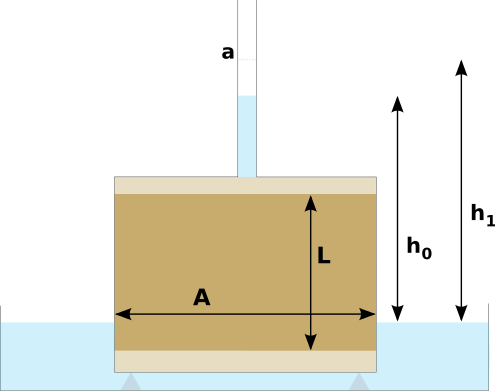
\includegraphics[scale=0.4]{darcy.png}
		\captionof{figure}{Schéma de l'équipement utilisé par Darcy pour obtenir l'équation \eqref{eq-Darcy-1}}
	\end{center}
\end{figure}

Il en déduisit une formule expérimentale
\begin{equation}
	\label{eq-Darcy-1}
	Q=KA\frac{\Delta H}{L}.
\end{equation}
$Q$ est le débit volumique s'écoulant à travers  
$A$ est la section du massif sableux\\
$\Delta H$ la perte de charge\footnote{En hydraulique la charge est une grandeur homogène à une longueur, on l'exprime parfois sous la forme d'une pression: $cste\times\rho g$. Elle est proportionnelle à l'énergie mécanique d'une molécule de fluide, on écrit \[H=\frac{v^2}{2g}+ z+ \frac{p}{\rho g}.\] Remarquons ici que la vitesse est considérée nulle.} de l'eau entre le sommet et la base du massif sableux\\
$K$ est une constante dépendant du milieu poreux, baptisée coefficient de perméabilité\\
$L$ est l'épaisseur du massif sableux.



\vspace{0.7cm}

On appelle $U=Q/A$ \textbf{la vitesse de filtration} d'un sol. À partir des équations de Navier-Stokes on sait que les causes du déplacement du fluide sont dues au gradient de pression ainsi qu'aux forces extérieures. La loi de Darcy s'exprime alors sous la forme générale
\begin{equation}
	\label{eq-Darcy}
	\overrightarrow{U}=\frac{k}{\mu }(\overrightarrow{\nabla}\, p+\rho g \,\overrightarrow{\nabla}\, z).
\end{equation} 

On peut réécrire cette équation
\[\overrightarrow{U}=-K(\overrightarrow{\nabla}\, h + \,\overrightarrow{\nabla}\, z),\]
avec $K=k(\mu \rho g)^{-1}$ $[LT^{-1}]$ et $h=p(\rho g)^{-1}$ $[L]$. On a donc 
\[H=h+z,\]
on peut alors injecter l'équation de Darcy \eqref{eq-Darcy} dans l'équation de conservation de la masse \eqref{eq-mass-por} pour finalement obtenir
\begin{equation}
	\label{eq-Richards}
 	-\overrightarrow{\nabla} \cdot (K\overrightarrow{\nabla}H)+\frac{\partial\theta}{\partial t}+ q=0.
\end{equation}  
On définit parfois des lois de porosité liées à la grandeur $f(H)=\theta$ la quantité d'eau est liée à la cote piézométrique \footnote{La cote piézométrique est l'altitude ou la profondeur (par rapport à la surface du sol) de la limite entre la nappe phréatique et la zone non saturée. Ce niveau est mesuré à l'aide d'un piézomètre.} et l'on pose 
\begin{equation}
	\label{eq-rapp-dens-H}
	S_s(H)\frac{\partial H}{\partial t}=\frac{\partial\theta}{\partial t},
\end{equation}
$S_s$ est appelé le coefficient d'emmagasinement. En supposant que $K$ est une fonction de $theta$ (nous avons expliqué que l'écoulement dépendait du rapport entre les forces de capillarité et celles gravitationnelles), ainsi en injectant l'équation \eqref{eq-rapp-dens-H} dans \eqref{eq-Richards} on obtient  \textbf{l'équation de Richard généralisée}
\begin{equation}
	\label{eq-ge-richard}
	S_s(H)\frac{\partial H}{\partial t}-\overrightarrow{\nabla} \cdot (K(\theta)\overrightarrow{\nabla}H)+q=0.
\end{equation}

Ceux sont avec ces équations que les hydrologues travaillent. Nous pouvons remarquer que cette simplification des équations peut être considérée comme le début d'un processus d'upscaling. On cherche à simplifier le modèle pour qu'il soit encore vrai à grand échelle. Notons que les équations de Darcy ont été justifiées dans les travaux de Matheron et Marle à partir de l'intégration dans un milieu réel des équations de Navier. 

\subsection{La problématique de l'upscaling dans l'étude des modèles hydrologiques}
\label{ch:modeles-hydro-upscaling}
Nous allons présenter dans cette partie deux modèles hydrologiques, le premier HydroGéoSphère, est celui que nous avons utilisé pour réaliser les modélisations hydrologiques sur le bassin du Little Washita. Le second, Orchidée est le modèle de surface continentale utilisé par l'IPSL. 

\subsubsection{Le modèle d'hydrogéosphère}

HydroGéoSphère (HGS) est un code de calcul hydrologique tri-dimensionnel, intégré et à base physique. Il a été développé par R. Therrien puis conjointement à l’Université de Laval, à Québec et à l’Université de Waterloo. Ce code de calculs permet de simuler les écoulements de surface et de subsurface, ainsi que le transport de solutés et d’énergie de manière intégrée, c’est-à-dire que les équations gouvernant ces processus sont résolues simultanément. Le code est parallélisé permettant une efficacité numérique élevée et donc des applications à des échelles spatio-temporelles importantes.

À chaque pas de temps le modèle résout les équations de transport d'eau de surface et de subsurface ainsi que celles conservation de la masse en même temps. En regardant la figure \ref{fig-HGS_water_balance} on a la conservation des quantités d'eau en surface s'écrit
\begin{equation}
	\label{eq-HGS-surface}
	P = (Q_{S2}-Q_{S1})-Q_{GS}+I+ET_S+Q^W_S+\Delta S_S /\Delta t,
\end{equation}
et les équations de subsurface s'écrivent
\begin{equation}
	\label{eq-HGS-subsurface}
	I = (Q_{G2}-Q_{G1})+Q_{GS}+ET_G + Q^W_G+\Delta S_G/\Delta t.
\end{equation}
On a finalement,
\begin{equation}
	\label{eq-HGS-bilan-tot}
	P=(Q_{S2}-Q_{S1})+(Q_{G2}-Q_G1)+(ET_S+ET_G)+(Q^W_S+Q_G)+(\Delta S+S+\Delta S_G)/\Delta t
\end{equation}
Avec $Q_{S1}$ et $Q_{S2}$ les flux entrant et sortant, $Q_{GS}$ le flot d'interaction entre la surface et la subsurface, $ET_S$ l'évapotranspiration de surface. $Q^W_S$ et $Q^W_G$ les termes puits définis précédemment \eqref{eq-mass-por}. $\Delta S_S$ et $\Delta S_G$ les différences de stockage d'eau en surface et en subsurface sur le temps $\Delta t$.

\begin{figure}[H]
	\begin{center}
		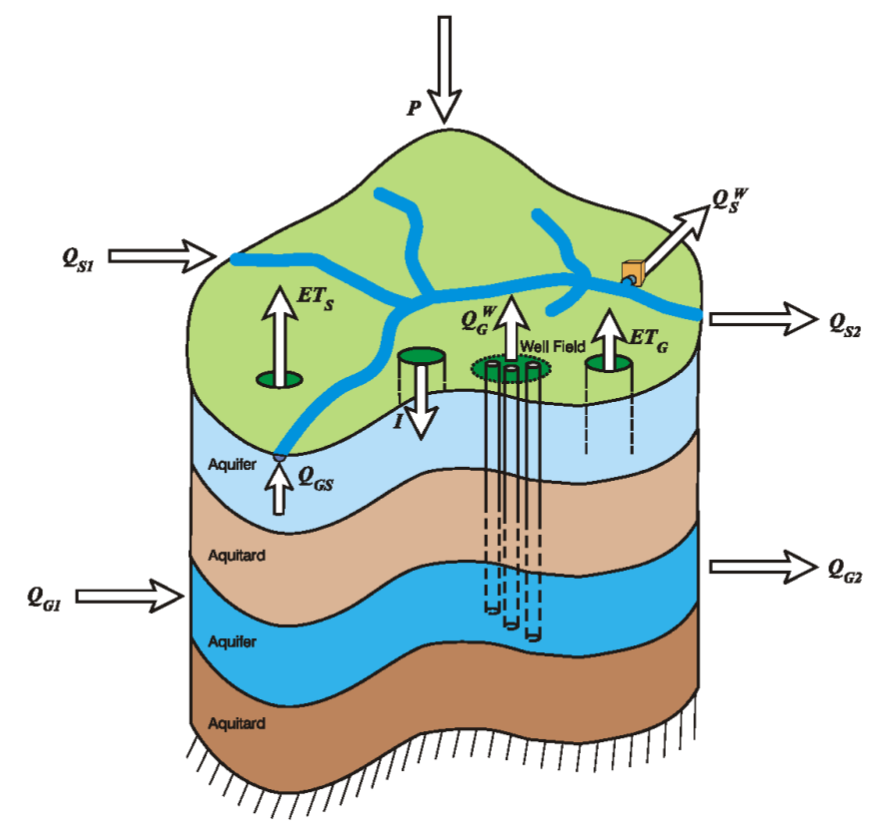
\includegraphics[scale=0.35]{HGS_modele.png}
	\end{center}
	\captionof{figure}{Schéma des cycles hydrologiques pris en compte par hydrogéosphère}
	\label{fig-HGS_water_balance}
\end{figure}

Hydrogésphère résout rigoureusement les équations de la physique cités dans la partie \ref{ch: eq meca-flu} et donne des résultats très précis. Cependant la capacité informatique actuelle ne permet pas d'implémenter HydroGéoSphère dans un modèle de climat. Il fallait donc créer des modèles plus simples et plus grossiers pour résoudre le problème à plus grande échelle. C'est le principe du modèle continentale Orchidée.

\subsubsection{Le modèle d'Orchidée}

Orchidée est un modèle continental dans le continuum sol-végétation-atmosphère. Ses résultats sont intégrés comme condition à la limite basse du modèle général de circulation atmosphérique du Laboratoire de Météorologie Dynamique. Orchidée simule en particulier les flux d’énergie, d’eau et de carbone entre les surfaces continentales et l’atmosphère. Il est composé de trois modules qui représentent des processus différents et agissant à des échelles de temps différentes: SECHIBA (Schématisation des Échanges Hydriques à l’Interface entre la Biosphère et Atmosphère), STOMATE, qui modélise principalement la phénologie végétale\footnote{La phénologie végétaleles étudie les phases de développement saisonnier des plantes liées au cycle climatique annuel et les échanges de carbone dans la biosphère.}. Dans le cadre de ce stage, seul le module SECHIBA a été étudié.

La description que nous allons en donner ici est très sommaire et rassemble ce que nous en avons compris de la discussion que nous avons eu avec Emmanuel Mouche et de la lecture de la présentation \cite{gumiberteau2016}. Le modèle d'Orchidée est un modèle de réservoir, c'est à dire qu'on discrétise l'espace en plusieurs zones qui peuvent contenir de l'eau. Nous avons vu qu'il y avait plusieurs types d'écoulements qui intervenaient à différentes échelles de temps et à différents endroits dans le sol. Orchidée considère alors trois types de transfert d'eau dans trois types de réservoirs. Les écoulements considérés sont: les écoulements de surface, de subsurface et finalement les échanges entre la rivière et la nappe. 

\begin{figure}[H]
	\label{fig-HGS}
	\begin{center}
		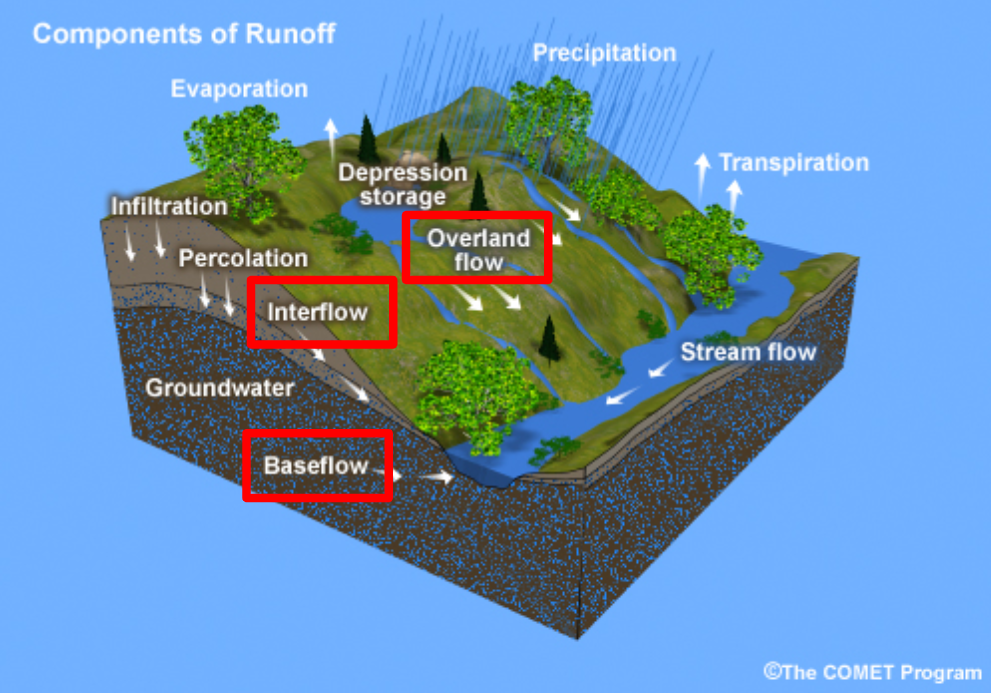
\includegraphics[scale=0.3]{different_flows.png}
	\end{center}
	\captionof{figure}{Schéma des cycles hydrologiques pris en compte par Orchidée (présentation \cite{gumiberteau2017})}
\end{figure}

La discrétisation de l'espace sera aussi par un maillage carré et l'on considérera pour chaque carré la découpe verticale du sol et l'on appelera ce volume un block. Orchidée discétise le sol par blocks. Alors dans chaque block considéré, il y a trois réservoirs d'eau. Un réservoir pour les écoulements de surface, un pour les écoulements de subsurface et un pour les interactions nappe-rivière (décrit dans la section \ref{ch:ecoulement}). La figure \ref{fig-Orchidee-interact} présente les intéractions entre deux blocks.

\begin{figure}[H]
	\begin{center}
		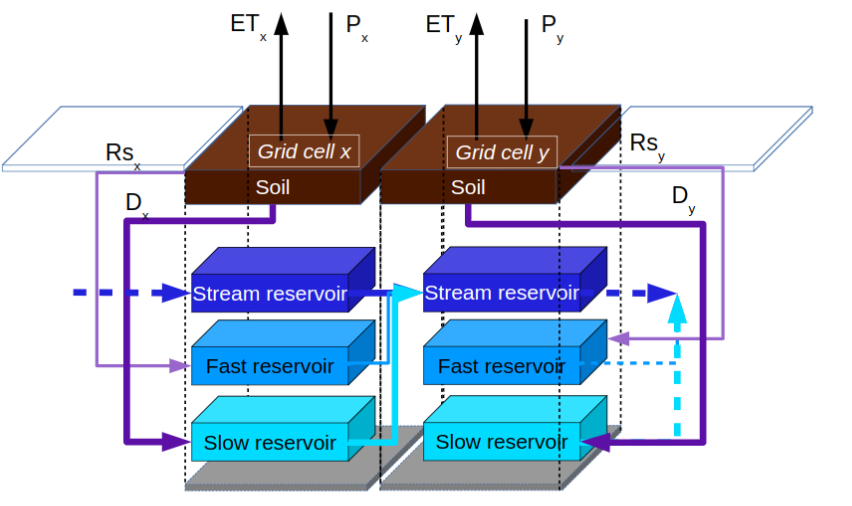
\includegraphics[scale=0.3]{Orchidee_interaction.png}
	\end{center}
	\captionof{figure}{Modèle de réservoir utilisé par Orchidée, image issue de \cite{gumiberteau2017}}
	\label{fig-Orchidee-interact}
\end{figure}

Remarquons que la couche du haut, dont nous n'avons pas parlé, est le sol sur lequel on considère les précipitations ($P_X$, $P_Y$) et l'évapotranspiration ($ET_X$,$ET_Y$). Le \textit{stream reservoir} est le réservoir des écoulements de surface, le \textit{fast reservoir} correspond au réservoir des écoulements de subsurfaces et le \textit{slow reservoir} correspond à la nappe. Les écoulements verticaux $(Rs_X,Rs_Y)$ et $(D_X,D_Y$) simulent les proportions des précipitations stockées dans chaque sous-block. Le calcul de $Rs$ et $D$ en fonction des précipitations est détaillé dans la présentation \cite{gumiberteau2017}. On peut remarquer que d'après ce schéma il n'y a pas d'écoulement de surface.
De plus, les écoulement ne vont que d'un réservoir à l'autre, ce paradigme semble raisonnable dans la mesure où les écoulements vont toujours dans le sens de la plus forte pente et ne se dispersent pas en général (le Nîl). Cependant, considérant la surface des blocks ($>0.5^{\circ}$), il est fréquent que plusieurs bassins soient contenus dans le même block, alors ce choix devient discutable.

\subsubsection{Questions ouvertes par la problématique de l'upscaling}

Ayant vu deux modélisations d'une surface continentale, leur comparaison peut enrichir la réflexion de l'upscaling. Voici ci-dessous les questionnements que nous avons eu par rapport à la problématique du downscaling

\begin{itemize}
	\item Quelles propriétés intéressantes voudrions nous pour les modèles upscalés? 
	\subitem Convergence du modèle upscalé lorsqu'on fait tendre la discrétisation vers $0$? 
	\subitem Majoration de la différence des grandeurs simulés par le modèle downscalé et les grandeur simulées par le modèle physique.   
	\item Comment quantifier la différence au modèle réel?
	\item Segmenter le modèle d'HydroGéoSphère en trois réservoir et regarder les bilans sur les différents réservoirs, puis injecter ces résultats dans le modèles Orchidée.
	\item Commencer par résoudre les équations de la physique dans chaque réservoir?
\end{itemize}

L'étude de ces questions pourrait faire l'objet d'un stage ou d'une thèse entière. 

\newpage
\section{Projections Climatiques et modélisation hydrologique sur le bassin versant du Little Washita}

\label{ch:proj-climatique-mod-hydro}

Dans cette section nous présentons les résultats que nous avons obtenus par l'analyse des données NARR sur le bassin du Little Washita. L'organisation de notre travail est résumée dans la figure \ref{fig-methodo}.

Commençons par rappeler les enjeux de ce stage. Nous cherchons à étudier l'impact du changement d'échelle sur les prédictions climatiques et les modélisations Hydrologiques. Avant de commencer notre travail, nous avons commencé par faire une étude de la région du Little Washita ainsi que des données NARR.

Pour étudier la problématique du changement d'échelle nous avons voulu étudier l'impact de différents changements d'échelles. Nous avons donc considéré des dégradations des données NARR sur plusieurs échelles (le processus de dégradation est expliqué dans la section \ref{ch:degradation-NARR}). On commence par considérer les variables de précipitation et d'évapotranspiration sur un point de maille NARR (le point couvrant la majeur partie du bassin du Little Washita) donc de $32km\times 32km$ puis nous avons considéré la moyenne des précipitations sur des ensembles de mailles entourant le point correspondant au Little Washita sur des surfaces de plus en plus grandes (voir section \ref{ch:degradation-NARR}).

Finalement, nous avons considéré le jeux de données du modèle de climat de l'IPSL qui possède une largeur de maille supérieur ($200km\times 200km$). Une fois récupérées les séries des réalisations des variables à ces différentes échelles nous avons appliqué la méthode CDFt pour les downscaler, donc transformer les données à grande échelle pour améliorer les projections sur la maille du Little Washita à petite échelle. Nous avons ensuite simulé la modélisation hydrologique pour toutes nos séries de précipitation et d'évapotranspiration. Enfin, nous avons étudié et comparé les résultats des débits renvoyés par les différentes simulations. Comme un schéma vaut mieux qu'un long discours voici celui résumant notre travail sur les données NARR en figure \ref{fig-methodo}.

\begin{figure}[H]
	\begin{center}
		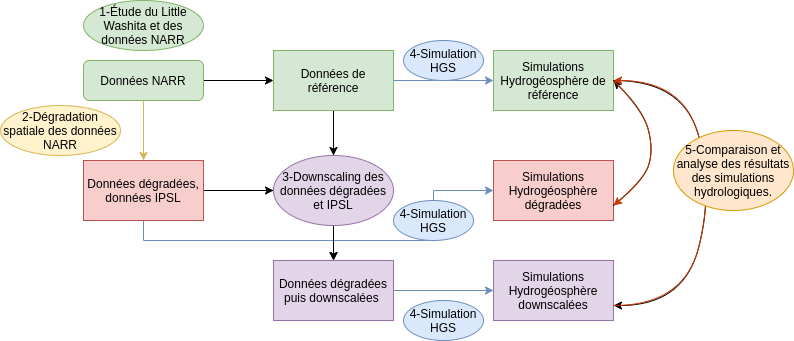
\includegraphics[scale=0.6]{Diagrame_methodo.png}
	\end{center}
	\captionof{figure}{Méthodologie d'étude du changement d'échelle}
	\label{fig-methodo}
\end{figure}

\subsection{Étude du Little Washita et des données NARR}

Nous allons donc étudier l'impact du changement d'échelle des données de précipitation et d'évapotranspiration (NARR, NARR dégradée et IPSL) sur la modélisation hydrologique du bassin versant du Little Washita. Nous avons décrit dans l'introduction quelques caractéristiques de ce bassin mais nous allons ici détailler la description de ce bassin. Nous préciserons ensuite les caractéristiques des données NARR.

\subsubsection{Le bassin versant du Little Washita}

Le bassin versant du Little Washita est situé dans l’État de l’Oklahoma, aux États-Unis. Ce bassin versant possède la particularité d’avoir fait l’objet de nombreuses études, dont les premières ont commencé dès les années 1930. Ces études ont permis d'avoir des données climatiques et hydrologique dans cette région dès les années 1960.

Ce bassin versant couvre une superficie d’environ $620 km^2$ . Sa topographie est qualifiée de modérément vallonnée \cite{allen1991hydrology}, avec une altitude variant de $320 m$ à $474 m$, avec une pente moyenne de $3,4 \%$ et une pente maximale d’environ $12 \%$. Le climat sur cette zone est tempéré continental\footnote{Les hivers froids et secs alternent avec des étés chauds et orageux, les saisons intermédiaires sont généralement de courte durée, aussi les amplitudes annuelles de températures importante. C'est au cours de l'été que tombent les pluies les plus abondantes.} \cite{rosero2011ensemble} et classé dans la catégorie ``subhumide'' selon la classification de Thornthwaite \cite{allen1991hydrology}. La température moyenne annuelle est de $16^{\circ}$ et la pluviométrie moyenne annuelle est d’environ $760 mm/m^2$. Cette température nous permet d'éviter de considérer les chutes de neige dans la modélisation hydrologique.

Le bassin versant est recouvert à environ $67\%$ de prairies (figure \ref{fig-little-washita-vegetation}). Les cultures constituent environ $20\%$ de la superficie et elles sont majoritairement localisées à proximité de la rivière. La surface restante est principalement recouverte de forêts et de quelques surfaces imperméables. 

\begin{figure}[H]
	\begin{center}
		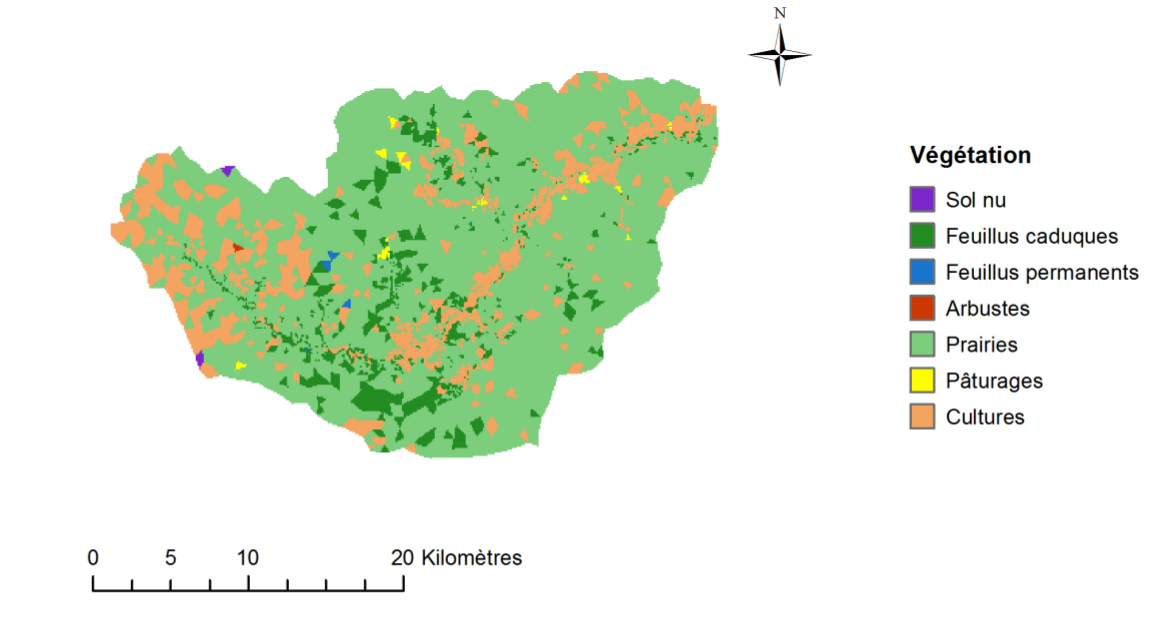
\includegraphics[scale=0.3]{vegetation_little_Washita.png}
	\end{center}
	\captionof{figure}{Carte de végétation du Little Washita (thèse \cite{maquin2016developpement})}
	\label{fig-little-washita-vegetation}
\end{figure}

\subsubsection{Les données North American Regional Reanalysis (NARR)}
\label{ch:NARR}

Les données NARR (North American Regional Reanalysis) couvrent l'entièreté du continent nord-américain et fournissent un total de $29$ variables climatiques. Pour les latitudes de $40^{\circ} N$ la longueure de grille est $32km$, ce qui en fait un maillage très précis. Les données NARR sont une extension du modèle NCEP Global Reanalysis couplées avec le système Regional Data Assimilation System (RDAS). Le premier modèle NCEP est un modèle de forçage climatique, c'est à dire un modèle climatique sur lequel on peut forcer les variables à avoir à certains temps et certaines positions (lieu et date des mesures) et RDAS un système utilisant à la fois les données satellites ainsi que les données récoltées sur terre pour fournir l'évaluation des variables climatiques avec grande précision. Les résultats climatiques résultant de cette association permettent de considérer les données NARR comme des données climatiques d'observation réelles, c'est à dire comme $\mathcal{T}$ définit dans l'équation \eqref{terre}. 

\begin{figure}[H]
	\begin{center}
		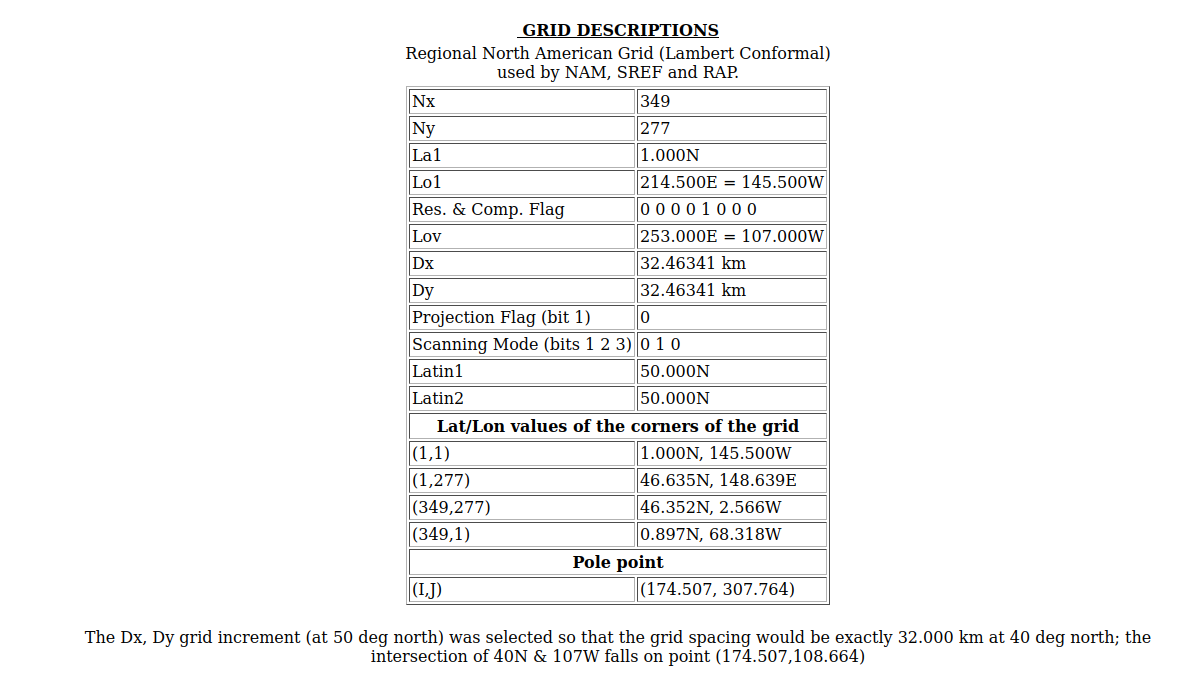
\includegraphics[scale=0.4]{grid_prop.png}
	\end{center}
	\captionof{figure}{Description du maillage NARR}
	\label{fig-maillage NARR}
\end{figure}

De plus, les données de chaque point sur terre $\mathcal{S}(\mathbb{R}^3)$ sont considérées comme des points dans l'espace $\mathbb{R}^2$. La méthode de cartographie utilisée par les données NARR est \textbf{la projection conique conforme de Lambert} (voir annexe \ref{proj-Lambert}). Nous allons considérer que la zone sur laquelle nous étudierons les données NARR est euclidienne, c'est à dire que la distance entre deux points adjacents du maillage est la même pour tous les couples de points adjacents du maillage (nous verrons dans l'annexe \ref{proj-Lambert} que cette approximation est raisonnable).

\vspace{0.7 cm}

Nous nous sommes limités à un sous ensemble des données NARR à savoir la région encadrant le Little Washita.
 

\begin{figure}[H]
	\begin{center}
		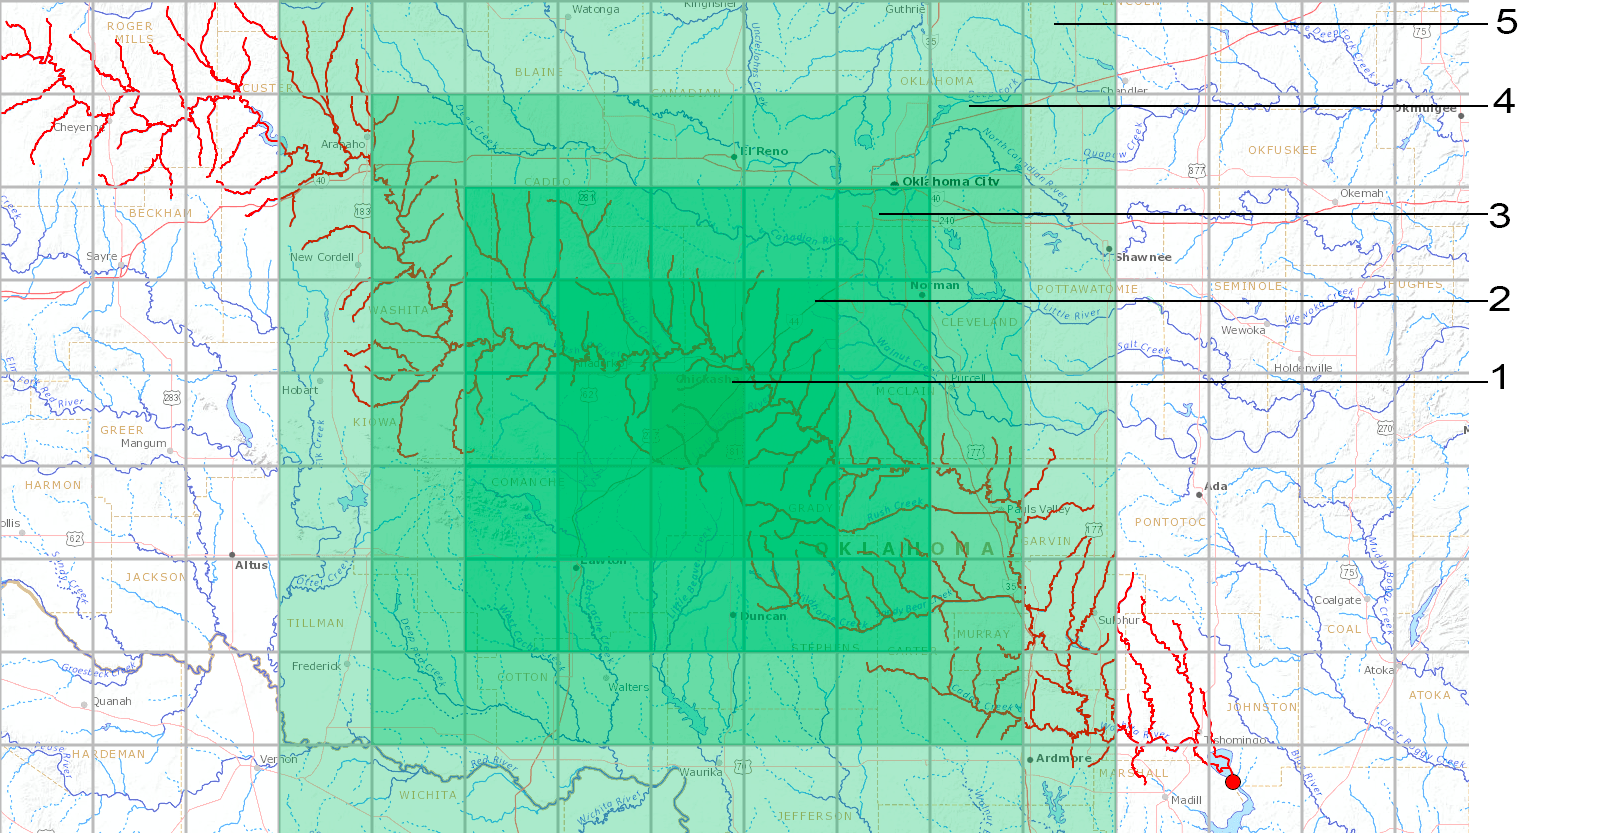
\includegraphics[scale=0.3]{Little_Washita.png}
	\end{center}
	\captionof{figure}{Visualisation du maillage considéré}
	\label{fig-Little-Washita_maillage}
\end{figure}

Sur chaque case de ce maillage, nous avons les données de précipitation et d'évaporation des années $1979$ à $2014$. Nous allons considérer par la suite le tenseur des données NARR $\mathcal{T}$ de dimension $T \times M\times N$ pour les deux variables considérées. $M$ et $N$ représentent les dimensions de l'axe vertical (latitudes) et horizontal (longitudes) de notre figure, et $T$ la période sur laquelle nous avons considéré nos dégradations. Nous voyons que la rivière du Little Washita (au centre du graphique) chevauche deux cases, on considère les variables sur la case couvrant la plus grande surface de la rivière comme case recouvrant le Little Washita.

\subsection{Dégradation spatiale des données NARR}
\label{ch:degradation-NARR}
Nous allons ici éclaircir ce que nous avons appelé la dégradation des données NARR dans les sections précédentes. L'on verra alors qu'il est intéressant d'analyser les variables de précipitation et d'évapotranspiration sur une zone plus large afin de mieux comprendre et anticiper les résultats de nos dégradations. 

\subsubsection{Méthode de dégradation}

En considérant de nouveau les données NARR comme un tenseur de dimension $T\times M \times N$,
nous avons dégradé les valeurs par un moyennage spatial. Nous avons fait $5$ dégradations différentes, on les numérote de $0$ à $4$, on appellera $\mathcal{T}^{d}$ le tenseur issu de la dégradation $d$, défini par
\begin{equation}
	\label{eq-degradation}
	\mathcal{T}^{d}{t,m,n}=\frac{1}{(2d+1)^2} \sum_{i=-d}^{d}\sum_{j=-d}^{d}\mathcal{T}_{t,m+i,n+j} \hspace{4mm} \forall (m,n) \in \{d+1,...,M-d\}\times\{d+1,...., N-d\}.
\end{equation}
On considère que le point de grille du Little Washita est le point $(0,0)$. 
\begin{definition}
	\label{serie-deg}
	Pour $d\geq1$, $(X^d_t)_{t\in \llbracket 1,T \rrbracket}$ les séries temporelles $\mathcal{T}^{d}_{0,0,t}$ sont appelées \textbf{séries dégradées}.
\end{definition}

Nous avons cherché à projeter la série $(Y_t)_{t \in \llbracket 1,T \rrbracket}= \mathcal{T}^{0}_{0,0,t}$ à partir des séries $(X^d_t)_{t\in \llbracket 1,T \rrbracket}$, $d\geq 1$ et ainsi regarder l'impact de la dégradation puis du downscaling sur les données.

\begin{figure}[H]
	\begin{center}
		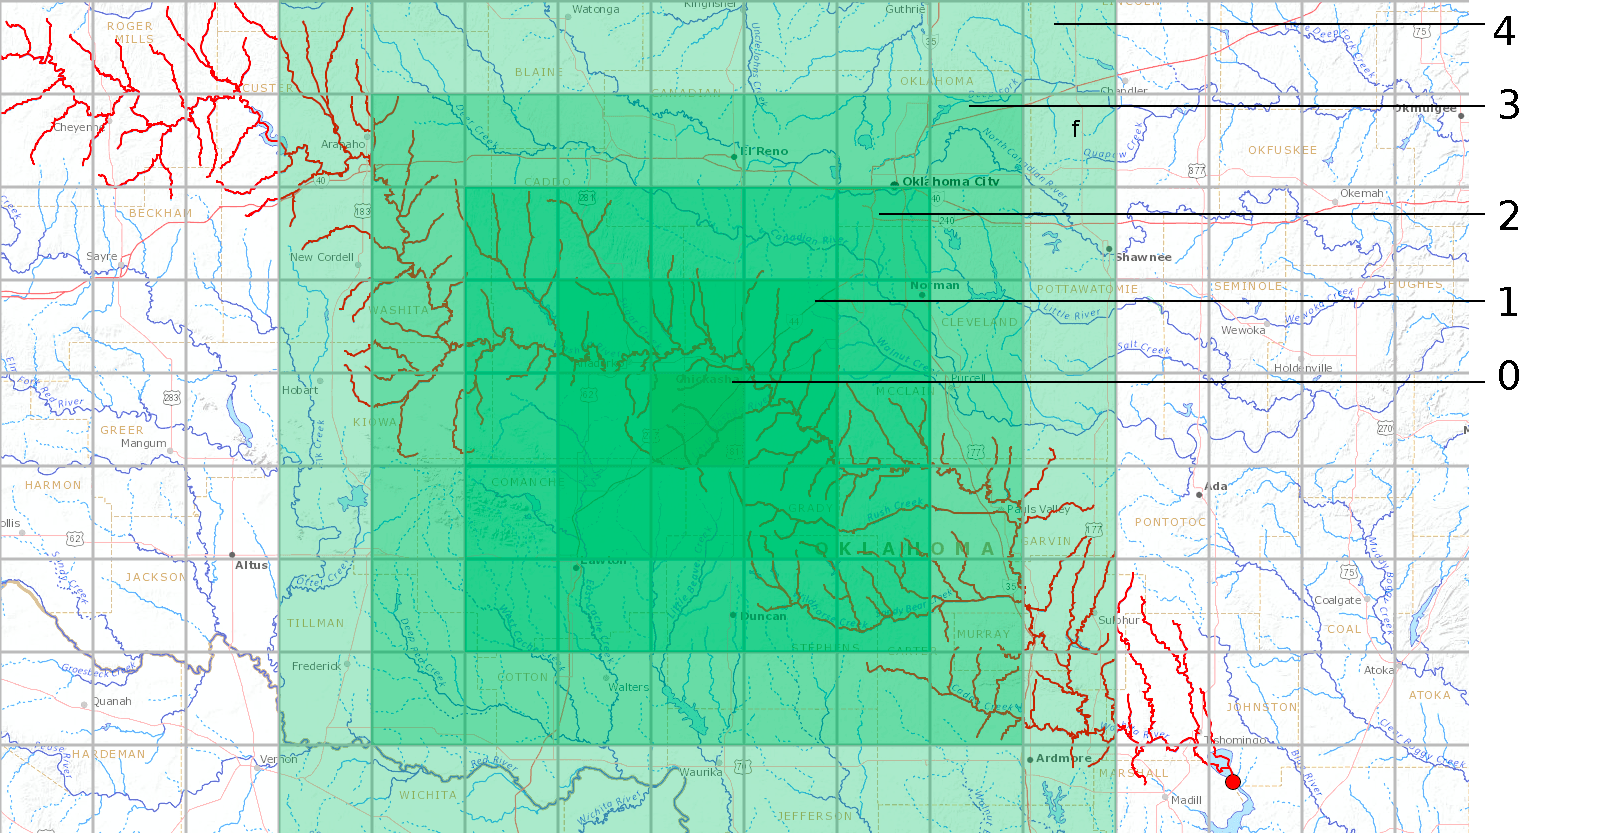
\includegraphics[scale=0.3]{Little_Washita_deg.png}
	\end{center}
	\captionof{figure}{Les différentes zones de dégradation considérées}
	\label{fig-Little-Washita-deg}
\end{figure}

Nous avons pour chaque $d$ dans $\{0,1,2,3,4\}$ la zone de dégradation correspondante à la dégradation $d$. Pour chaque $d$, $(X^d_t)$ vérifie l'égalité 
\[X^d_t=\frac{Y_t}{(d+1)^2}+ G^d_t,\]
où $G^d_t$ est une variable aléatoire proportionnelles à la somme des réalisations des voisins du point de grille du Little Washita $(0,0)$. On sait dans ce cas là que $Y_t$ est ``contenue'' dans $X^d_t$, ce qui peut avoir un impact sur downscaling. Dans le cas des données IPSL, les données ne sont pas nécessairement corrélées. Nous allons donc regarder l'efficacité du donscaling pour les différentes dégradations ainsi que pour les données de l'IPSL.

\subsubsection{Analyse spatiale de la région du Washita}
\label{ch:analyse spatiale Washita}

Pour les deux variables, nous allons regarder leur valeurs moyennes sur les années $1979-2014$ pour les différents points de grilles entourant le little Washita. Dans les prochains graphiques l'axe $X$ sera l'axe de la dimension $M$ (la latitude) et l'axe $Y$ celui de $N$ (la longitude). Les coordonnées du Little Washita seront encore $(0,0)$.

\begin{figure}[H]
	\begin{center}
		\begin{minipage}[b]{0.49\linewidth}
			\centering 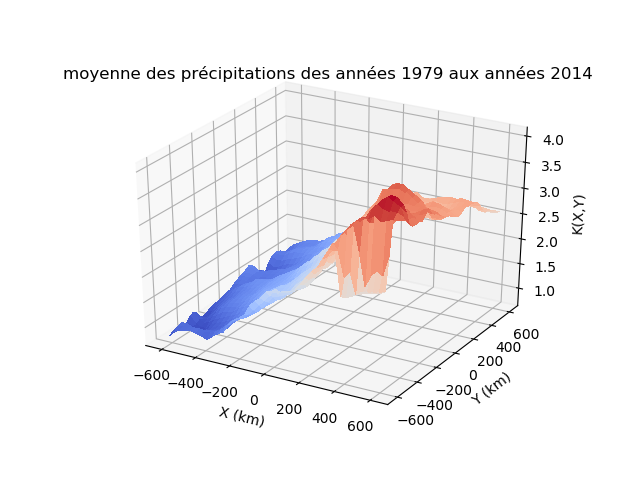
\includegraphics[scale=0.5]{images/mean_precip.png}
		\end{minipage}\hfill
		\begin{minipage}[b]{0.49\linewidth}	
			\centering 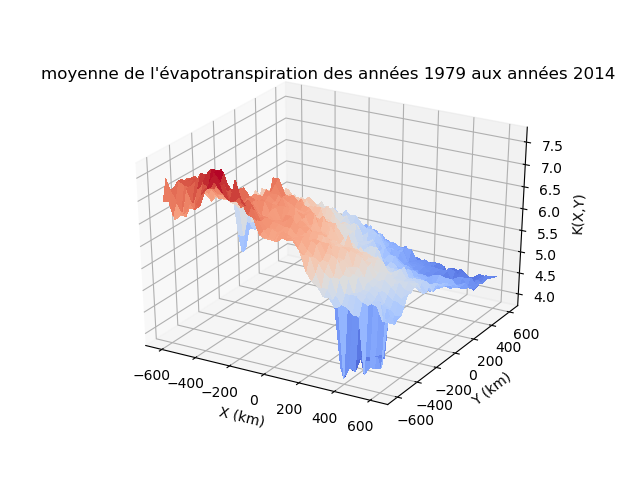
\includegraphics[scale=0.5]{images/mean_evap.png}
		\end{minipage}
	\end{center}
	\caption{Tracé des précipitations($mm.m^{-2}.j^{-1}$) et de l'évapotranspiration($mm.m^{-2}.j^{-1}$) moyenne de $1979$ à $2014$}
\end{figure} 
Nous voyons que les moyennes des précipitation sont de plus en plus faible à mesure que l'on descend vers l'équateur. La pente parait tout de même très importante. En revanche on voit qu'au point $(0,0)$ la précipitation journalière moyenne est d'environ $2mm$ ce qui correspond à peu près aux $760 mm/m^2$ trouvés par \cite{allen1991hydrology}. Il semble que le gradient moyen de l'évapotranspiration potentielle soit orienté vers le Sud-Est. La considération de ces deux graphique semble cohérente avec la désertification dans le sud des états Unis et les grandes plaines du Nord des États Unis.

\vspace{0.7cm}

On s'intéresse maintenant à la structure de covariance spatiale de nos données. Tout d'abord, $\mathcal{T}_{V}$ possède une fonction de covariance spatiale car les réalisations des ses variables sont bornées. Il est habituel de faire des hypothèses sur cette fonction de covariance afin de pouvoir la manipuler et l'interpréter plus simplement. On appelle cette fonction de covariance $K$ on l'appelle habituellement noyau de covariance.

\begin{definition}
	Soit $f:\mathbb{R}^{+}\times\mathbb{R}^2\to \mathbb{R}$ une fonction aléatoire, on définit un noyau de covariance sur cette fonction en faisant l'hypothèse que $f$ est stationnaire en temps et espace, on a alors
	\[Cov(f(t,x),f(t,x+y))=K(y), \hspace{4mm} \forall t \in \mathbb{R}^{+},\,x,y \in \mathbb{R}^2. \] 
\end{definition}

On remarque de plus que la fonction $K$ ainsi définie est symétrique, $K(y)=K(-y),\, \forall y \in \mathbb{R}^2$. On peut alors simplement calculer la covariance empirique à partir de l'estimateur sans biais de la variance.

\[K(m,n)=\frac{1}{T(M-m+1)(N-n+1)-1}\sum_{t=1}^{T}\sum_{i=m}^{M}\sum_{j=n}^{N}(\mathcal{T}_{t,i,j}-\overline{\mathcal{T}}_{1,m,n})(\mathcal{T}_{t,i-m,j-n}-\overline{\mathcal{T}}_{2,m,n}),\]
où,
\[\overline{\mathcal{T}}_{1,m,n}=\frac{1}{T(M-m+1)(N-n+1)}\sum_{t=1}^{T}\sum_{i=m}^{M}\sum_{j=n}^{N}(\mathcal{T}_{t,i,j}),\]
et 
\[\overline{\mathcal{T}}_{2,m,n}=\frac{1}{T(M-m+1)(N-n+1)}\sum_{t=1}^{T}\sum_{i=0}^{M-m}\sum_{j=0}^{N-n}(\mathcal{T}_{t,i,j}).\]
On peut donc tracer le noyau de covariance $K(i,j)$, $i \in\{-N/2,N/2\}$, $j \in \{-M/2,M/2\}$. 

\vspace{0.7cm}

\noindent \textbf{Résultats:}

Pour obtenir nos résultats, nous avons pris en compte la saisonnalité. En effet, nous avons séparé notre tenseur $\mathcal{T}$ en $12$ tenseurs sur chaque mois de l'année. On a donc pour chaque série downscalé 12 fois selon chaque mois. Voici les résultats obtenus en fonction des mois de l'année:

\begin{figure}[H]
\hspace{-1.3cm}
\begin{tabular}{ccc} 
	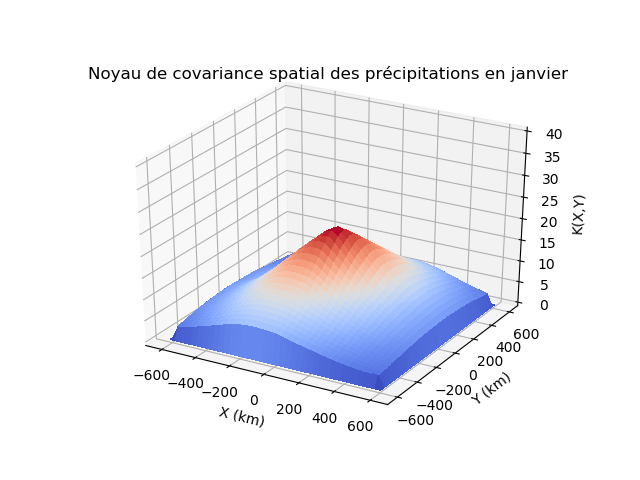
\includegraphics[scale=0.34]{images/kernel_precip_m1.png} & 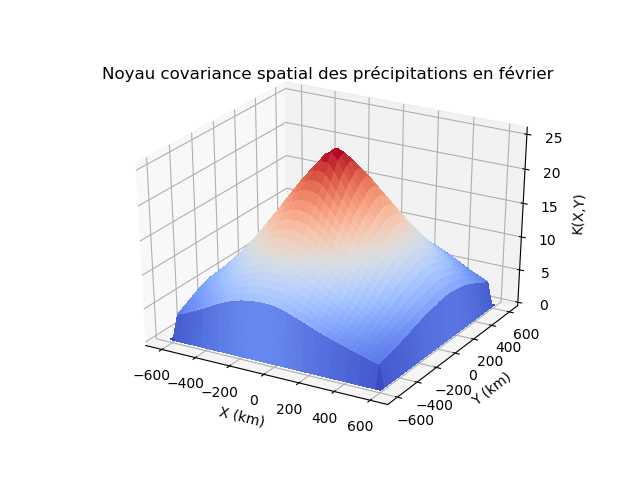
\includegraphics[scale=0.34]{images/kernel_precip_m2.png} & 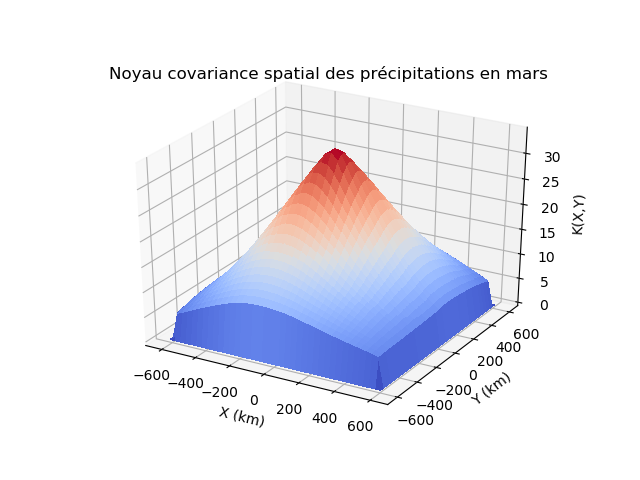
\includegraphics[scale=0.34]{images/kernel_precip_m3.png} \\ 
	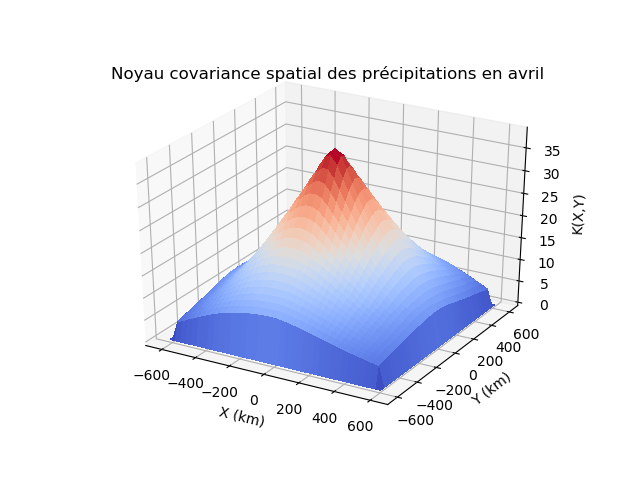
\includegraphics[scale=0.34]{images/kernel_precip_m4.png} & 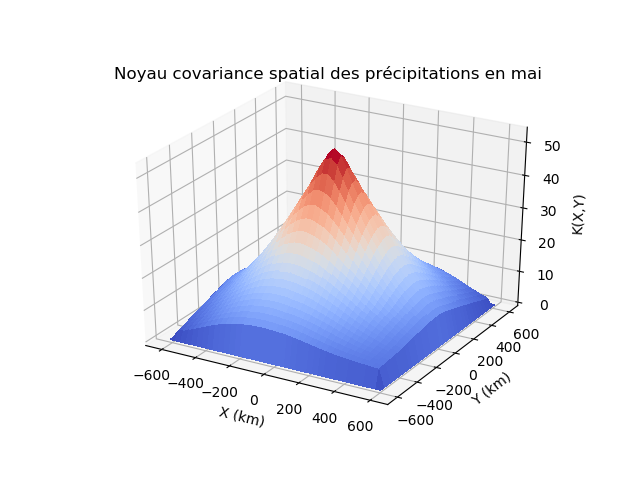
\includegraphics[scale=0.34]{images/kernel_precip_m5.png} & 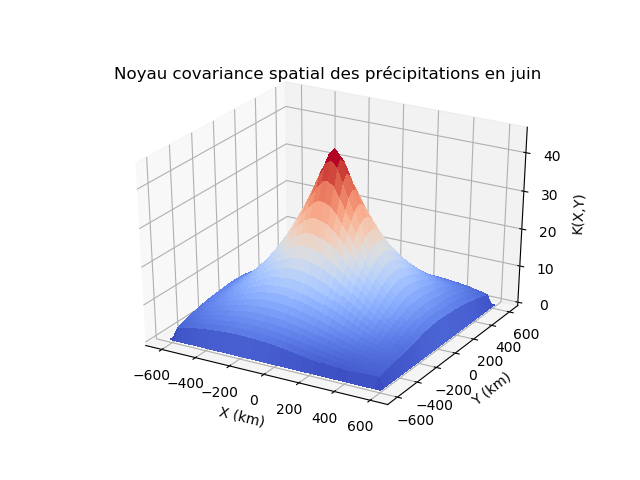
\includegraphics[scale=0.34]{images/kernel_precip_m6.png} \\
\end{tabular}

\hspace{-1.3cm}
\begin{tabular}{ccc}
	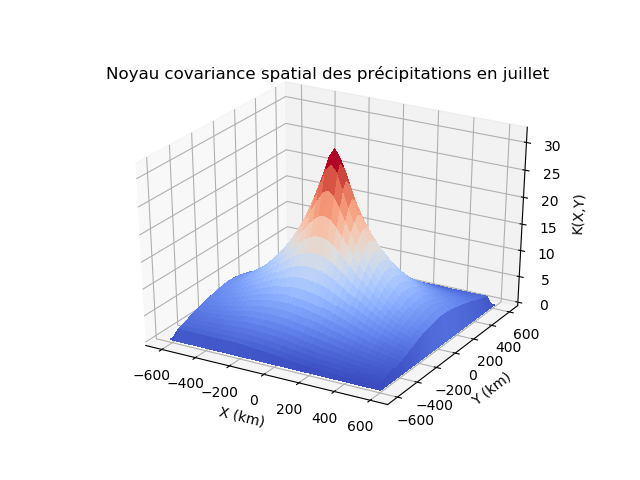
\includegraphics[scale=0.34]{images/kernel_precip_m7.png} & 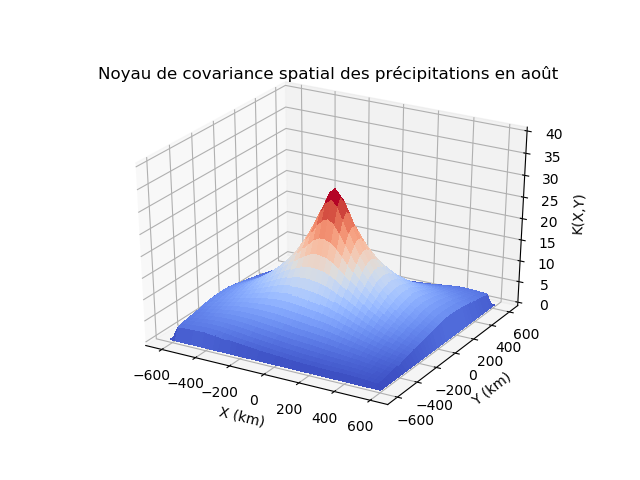
\includegraphics[scale=0.34]{images/kernel_precip_m8.png} & 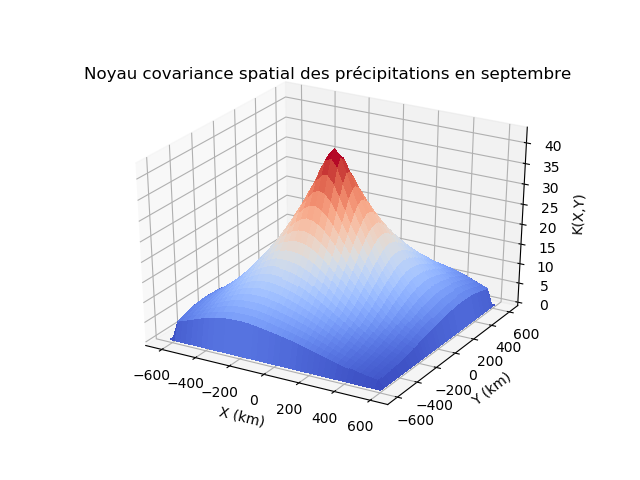
\includegraphics[scale=0.34]{images/kernel_precip_m9.png} \\ 
	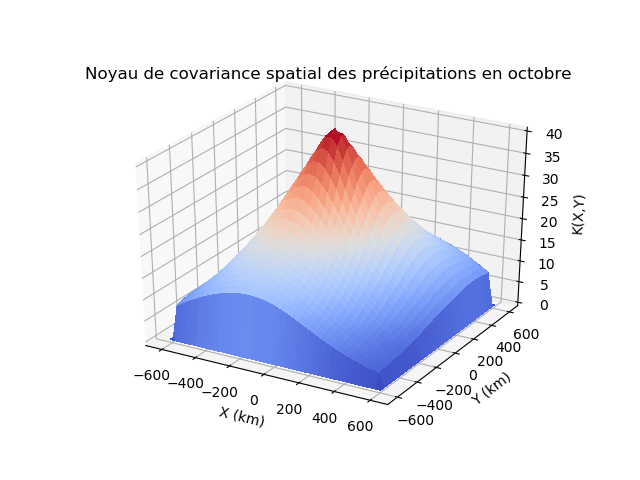
\includegraphics[scale=0.34]{images/kernel_precip_m10.png} & 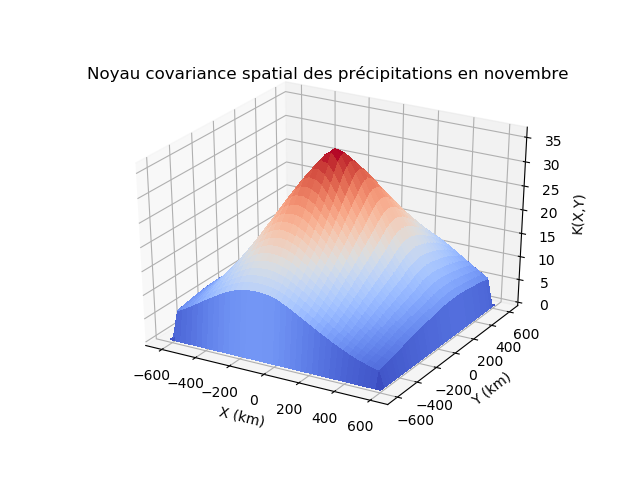
\includegraphics[scale=0.34]{images/kernel_precip_m11.png} & 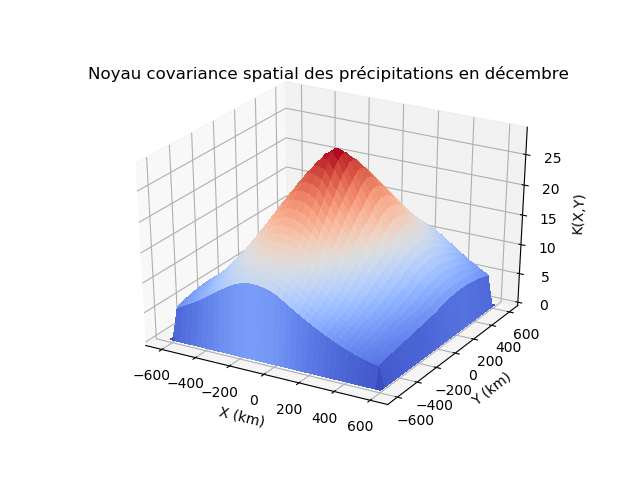
\includegraphics[scale=0.34]{images/kernel_precip_m12.png} \\
\end{tabular}
	\label{fig-kernel-precip}
	\caption{Noyau de covariance des précipitations en fonction des différents mois de l'année}
\end{figure}

D'après la figure 16, nous voyons qu'en été la covariance entre deux points s'effondre relativement vite alors qu'en hiver c'est plutôt l'inverse. Ce résultat était attendu car en été la plus est essentiellement convective, donc très locale, alors qu'en hiver c'est plus lié à des structures stratiformes à grande échelle donc plus similaire spatialement (c.f. \ref{ch:precipitations}).
Il est intéressant de constater que même à plusieurs centaines de kilomètres il y a encore une covariance entre les précipitations. On voit aussi que la covariance spatiale des précipitations diminue plus vite selon les latitudes. Ces phénomènes sont liés aux types de nuages qui dépendent des saisons.

\begin{figure}[H]
	\label{fig-kernel-evap}
\hspace{-1.3cm}
\begin{tabular}{ccc} 
	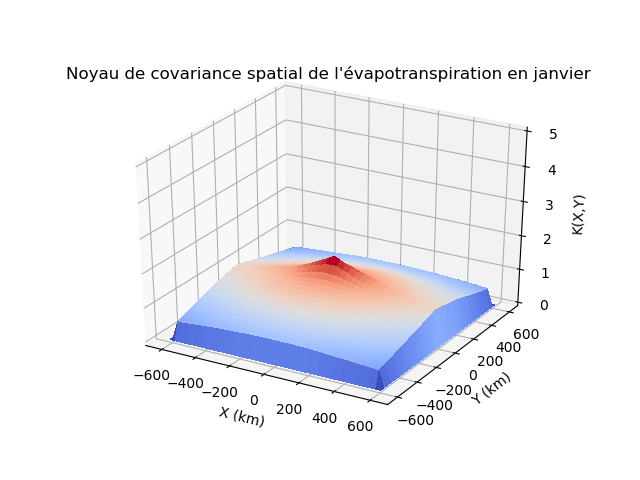
\includegraphics[scale=0.34]{images/kernel_evap_m1.png} & 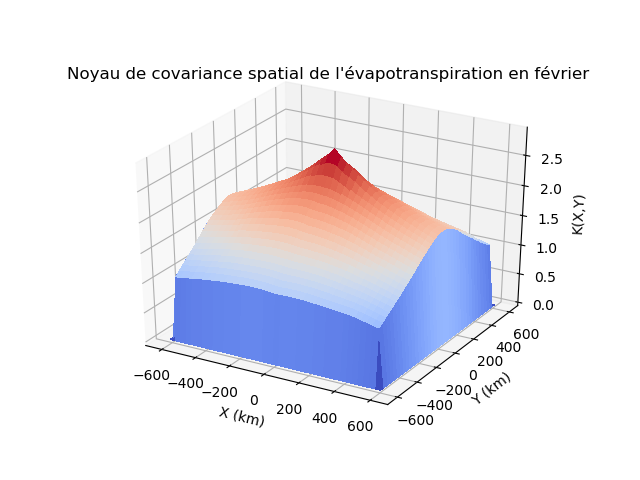
\includegraphics[scale=0.34]{images/kernel_evap_m2.png} & 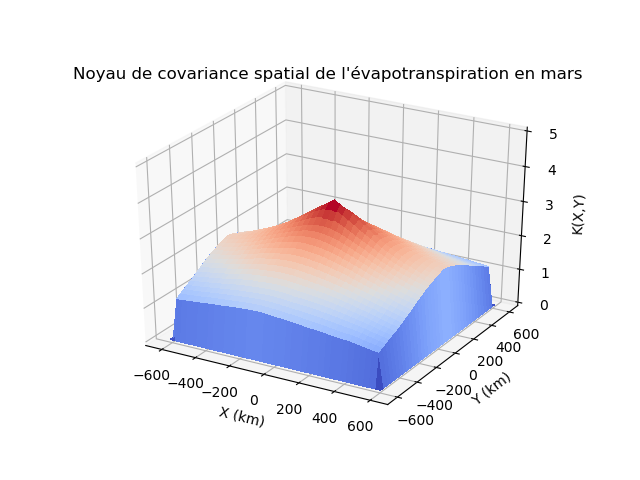
\includegraphics[scale=0.34]{images/kernel_evap_m3.png} \\ 
	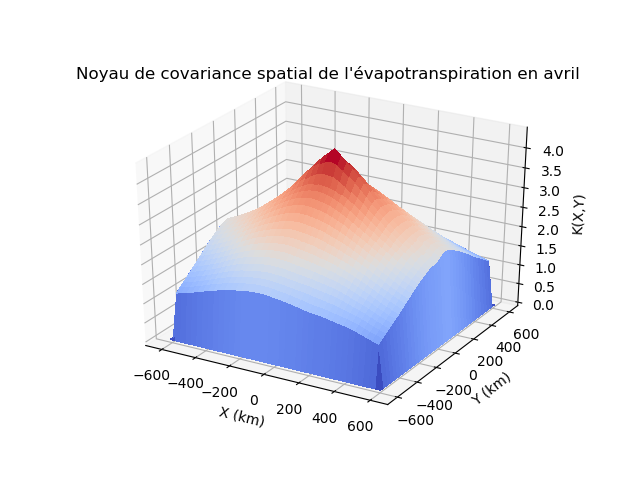
\includegraphics[scale=0.34]{images/kernel_evap_m4.png} & 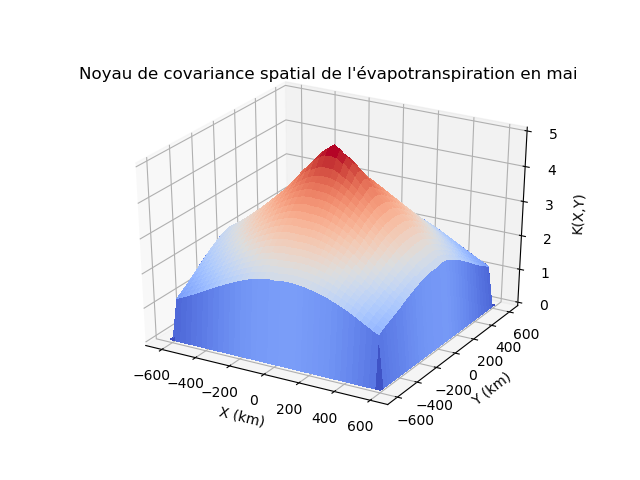
\includegraphics[scale=0.34]{images/kernel_evap_m5.png} & 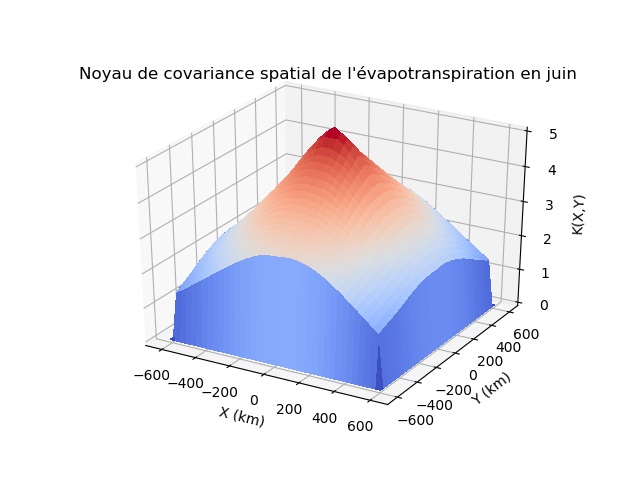
\includegraphics[scale=0.34]{images/kernel_evap_m6.png} \\
\end{tabular}

\hspace{-1.3cm}
\begin{tabular}{ccc}
	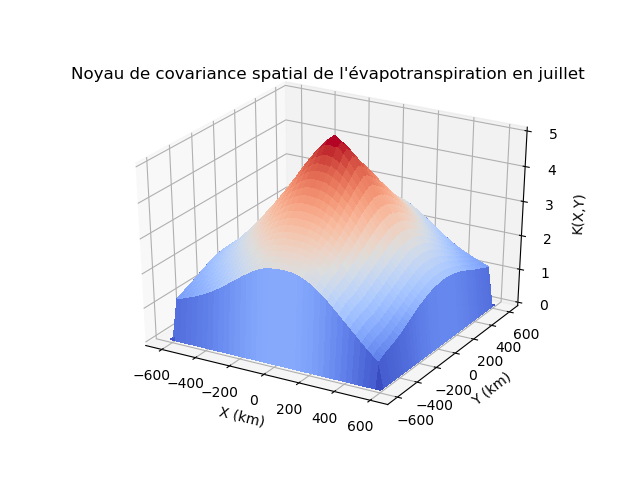
\includegraphics[scale=0.34]{images/kernel_evap_m7.png} & 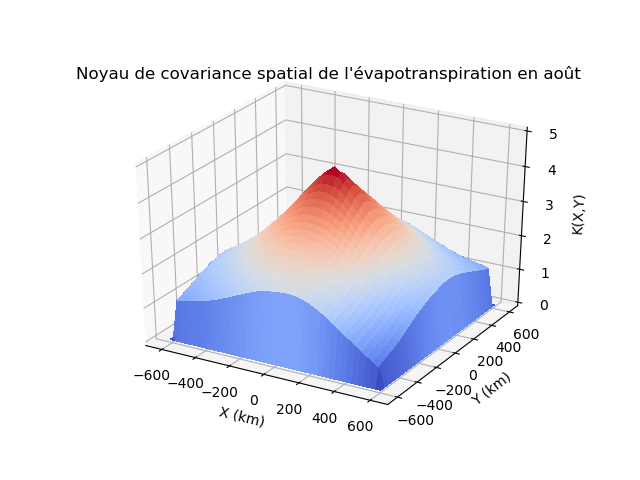
\includegraphics[scale=0.34]{images/kernel_evap_m8.png} & 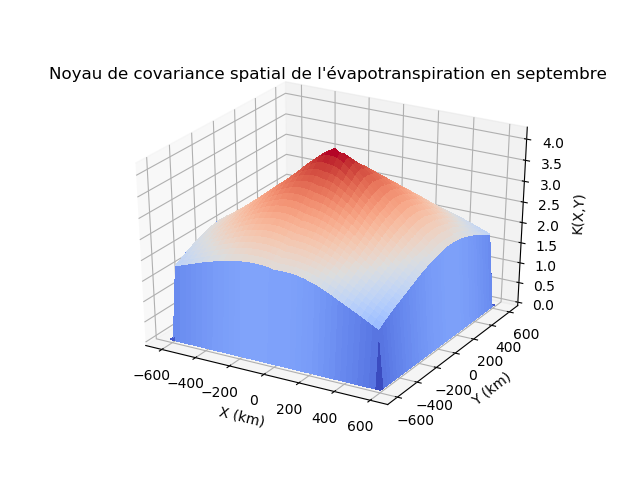
\includegraphics[scale=0.34]{images/kernel_evap_m9.png} \\ 
	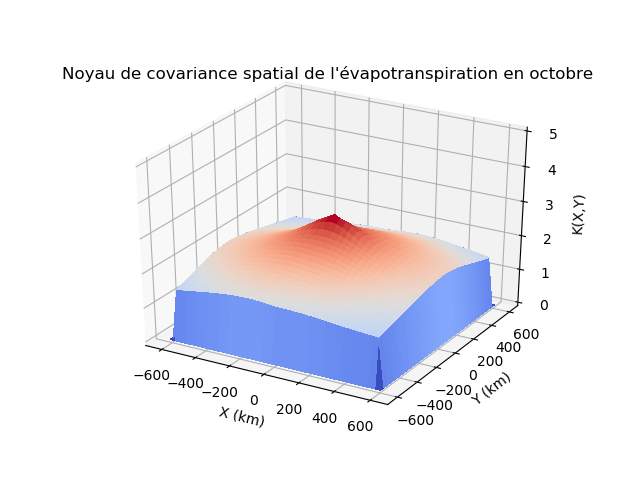
\includegraphics[scale=0.34]{images/kernel_evap_m10.png} & 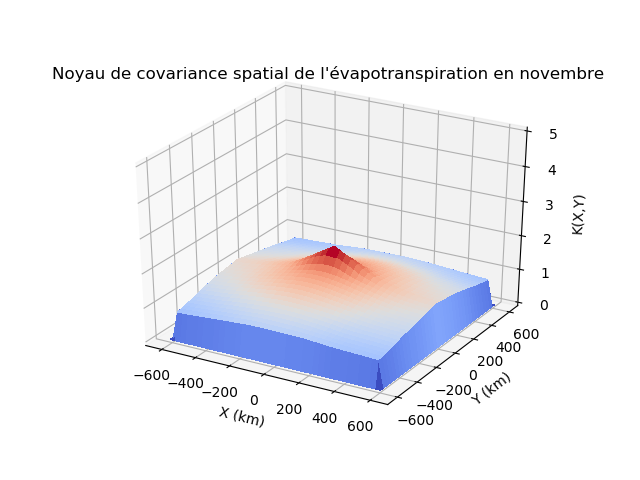
\includegraphics[scale=0.34]{images/kernel_evap_m11.png} & 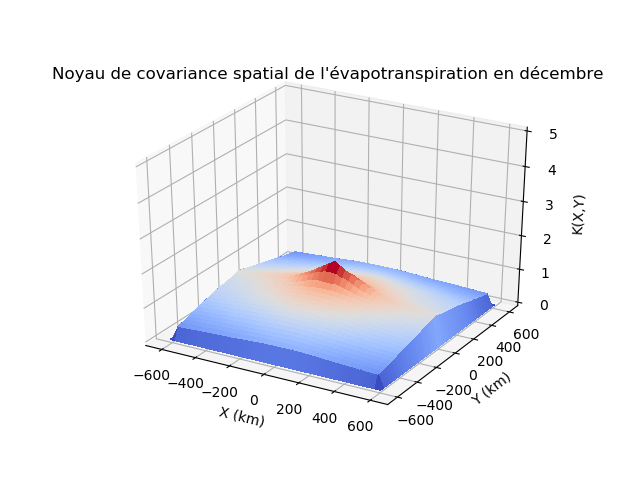
\includegraphics[scale=0.34]{images/kernel_evap_m12.png} \\
\end{tabular} 
	\caption{Noyau de covariance de l'évapotranspiration potentielle en fonction des différents mois de l'année}
\end{figure}

Dans la figure 17, nous voyons que la variance est aussi liée à la saisonnalité et que la variance semble diminuer moins vite selon la distance pour l'évapotranspiration que pour les précipitations. La variance est, elle beaucoup plus faible que pour les précipitations ($\sim 10 \times$ moins). 

\subsection{Downscaling des données dégradées et des données IPSL}
\label{ch:downscaling des donnees}

Maintenant que nous avons une idée de la structure spatiale des données NARR, nous allons dégrader puis downscaler les données dégradées et étudier les résultats obtenus. Pour nous remettre en tête les problématiques du downscaling on rappelle que les processus stochastiques $(X^d_t)_{t\in T}$ sont des estimateurs de $(Y_t)=\mathcal{T}_{t,0,0}$. Nous allons considérer les données journalières des précipitations et de l'évapotranspiration sur la période allant de $1979$ à $1996$ comme données d'apprentissage pour définir la transformation $G$ définie dans la partie \ref{ch:CDFt}.

Nous avons essayé plusieurs versions CDFt avec des méthodes utilisant des prédictions sur la moyenne et la covariance, comme expliquée dans la section \ref{ch:CDFt}. Cependant, les résultats n'ont pas été convaincants. Après plusieurs tentatives, l'algorithme CDFt le plus convaincant au sens de la distance de Cramér-von Mises était finalement celui où l'on effectuait aucune transformation, c'est à dire, celui où l'on utilisait la transformation du quantile-quantile sur les données. Néanmoins, nous verrons que cette transformation sous-estimait les derniers quantiles.

Il resterait très intéressant de développer et de tester les idées énoncées dans la partie \ref{ch:downscaling} car les résultats du quantile-quantile ne prennent pas en compte l'évolution du support des variables $X^d$ (les résultats obtenus ont montré que la dilatation n'est certainement pas la meilleure option).

Finalement, les résultats utilisés et étudiés par la suite sont les résultats obtenus par l'algorithme CDFt-SSR (voir ??Y a-t-il une source??) fourni par Mathieu Vrac pour les données de précipitation, et ceux de l'algorithme CDFt (voir \cite{vrac2012dynamical}) fourni par Mathieu Vrac pour l'évapotranspiration. Nous expliquerons ce choix dans ce qui va suivre.

\subsubsection{Analyse variationnelle des différentes séries de projection de la précipitation}
\label{ch:analyse variationnelle}
On commence par afficher un boxplot des différentes séries observées. Nous avons ainsi les boxplot pour la précipitation et l'évapotranspiration pour juger de la répartition des points pour chaque série.

\begin{figure}[H]
	\begin{minipage}[b]{0.48\linewidth}
		\centering 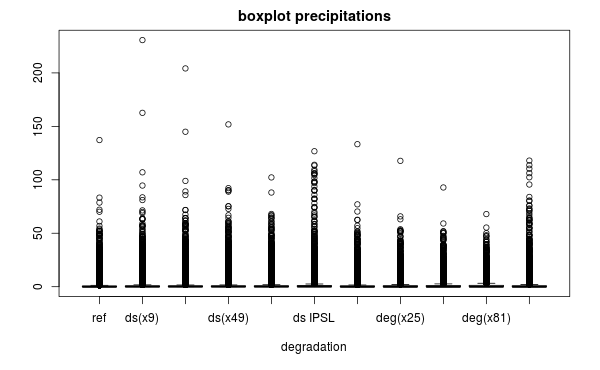
\includegraphics[scale=0.4]{images/boxplot_precip.png}
	\end{minipage}\hfill
	\begin{minipage}[b]{0.48\linewidth}	
		\centering 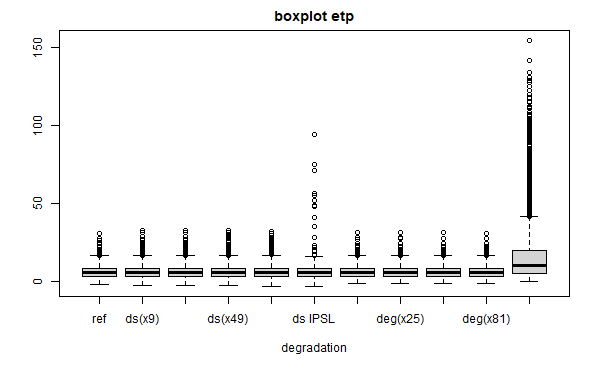
\includegraphics[scale=0.4]{images/boxplot_evap.png}
	\end{minipage}
	\caption{Boxplot en fonction des séries pour la précipitation et l'évapotranspiration}
\end{figure} 

Les colonnes représentent pour chaque variable:
\begin{itemize}
	\item 1- la série de observée sur le Little Washita $(Y_t)_{t\in T}$. 
	\item 2-3-4-5- Les séries downscalées des dégradations $(X^d_t)_{t \in T}$, $d \in \{1,2,3,4\}$.
	\item 6- La série downscalée de l'IPSL. 
	\item 7-8-9-10- Les séries des dégradations $d \in \{2,3,4,5\}$.
	\item 11- La série de l'IPSL. 
\end{itemize}
On voit que la dégradation de l'évapotranspiration n'a quasiment aucune influence sur les séries temporelle, ce qui était à prévoir d'après le noyau de covariance que nous obtenu précédemment (figure 17) pour l'évapotranspiration. On peut aussi voir que le modèle de climat de l'IPSL projette relativement mal l'évapotranspiration sur la région du Little Washita. Le downscaling dans ce cas là améliore nettement les résultats.

\subsubsection{Étude du downscaling sur la correction de biais}

D'après les boxplot il semble que plus la dégradation est grande, plus on sous-estime les données. Nous allons afficher les précipitations projetées (dégradée ou dégradées puis downscalées) en fonction des précipitations réelles. Cette méthode, permet de juger visuellement de l'efficacité du downscaling sur les données. Les figures qui sont affichées en dessous ont un titre indiquant le degré de déformation dans leur titre sous la forme $(2d+1)^2$ où $d$ est le degré dans l'équation de dégradation \eqref{eq-degradation}. Les figures de gauches sont les figure dégradées puis downscalées et celles de droites les figures dégradée, une ligne correspond à la même dégradation.	

\vspace{0.7cm}

\begin{figure}[H]
	
	\centering
	\begin{subfigure}[b]{0.45\textwidth}
		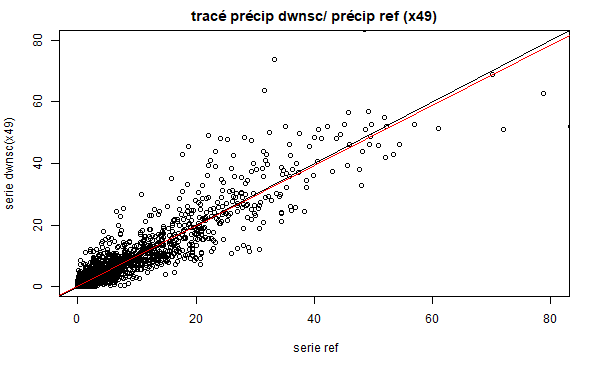
\includegraphics[scale=0.35]{images/pr_3_CDFt_ref.png}
	\end{subfigure}
	\hfill
	\begin{subfigure}[b]{0.45\textwidth}
		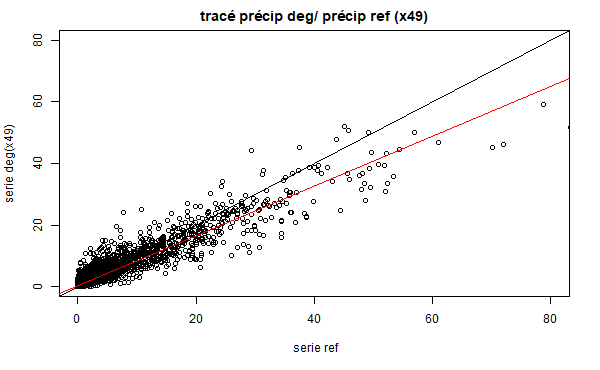
\includegraphics[scale=0.35]{images/pr_3_dg.png}
	\end{subfigure}
	\begin{subfigure}[b]{0.45\textwidth}
		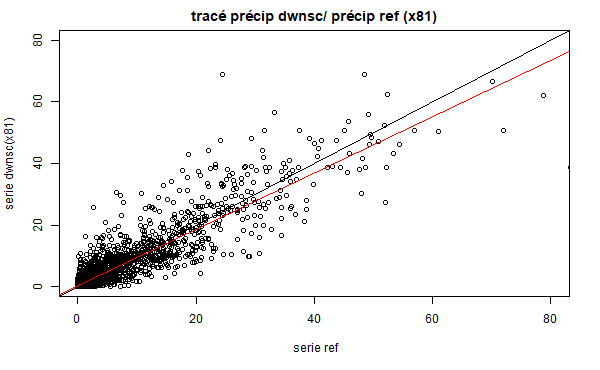
\includegraphics[scale=0.35]{images/pr_4_CDFt_ref.png}
	\end{subfigure}
	\hfill
	\begin{subfigure}[b]{0.45\textwidth}
		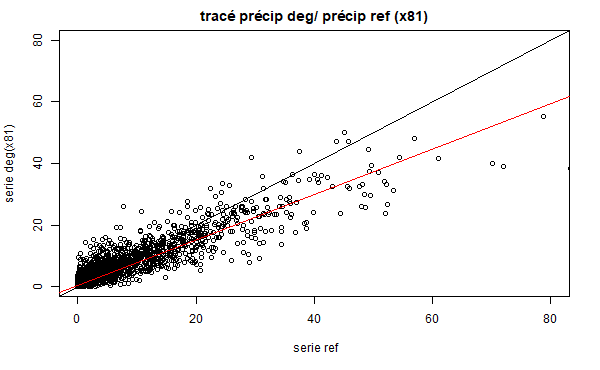
\includegraphics[scale=0.35]{images/pr_4_dg.png}
	\end{subfigure}
	\caption{Tracé des précipitations downscalées (CDFt) en fonctions des précipitations de référence pour les dégradations $3$ et $4$}
\end{figure} 

Visuellement, il semble que le downscaling améliore les projections. Nous avons tracé pour chaque figure en noire la droite identité et en rouge les droites de régression linéaire de la forme $y=ax+b$, où $x$ est la précipitation de référence et $y$ la donnée projetée de $x$. Dans notre cas c'est soit la dégradation $(X'^d_t)$, soit son downscalé $G_{X^d,Y}(X'^{d}_t)$. Remarquons que la dégradation de nos données ne crée pas de changement important de l'éparpillement des points dans les graphiques, c'est en accord avec les figures obtenues dans la section \ref{ch:analyse spatiale Washita} montrant une relativement grande covariance spatiale. Il semble cependant que la dégradation ait une tendance à sous-évaluer les précipitations élevées, ce qui ne semble pas aberrant si l'on considère les tailles des cumulonimbus\footnote{Les cumulonimbus sont des nuages très hauts se formant à partir des mouvements convectifs d'air chaud en été et leur taille va de $2$ à $10$km de diamètre.}, inférieur à la largeur de grille des données NARRs ($32$km). Alors on peut considérer les précipitations importantes comme des évènements localisés sur un seul point de grille NARR.


\subsubsection{Analyse des séries downscalées et explication du choix de la méthode de downscaling}

\begin{figure}[H]
	\label{fig-res_CVM_CDFt}
	\centering
	\begin{subfigure}[b]{0.45\textwidth}
		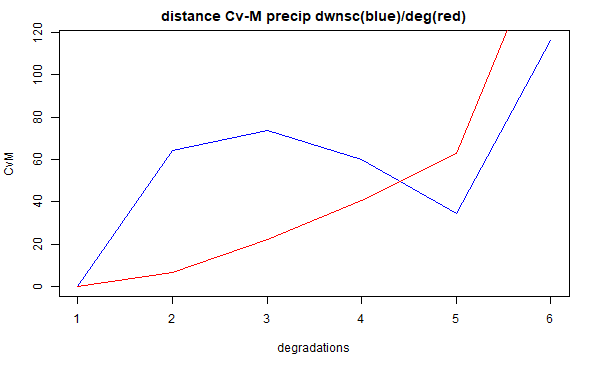
\includegraphics[scale=0.4]{images/Dist_CVM_precip_CDFt.png}
	\end{subfigure}
	\hfill
	\begin{subfigure}[b]{0.45\textwidth}
		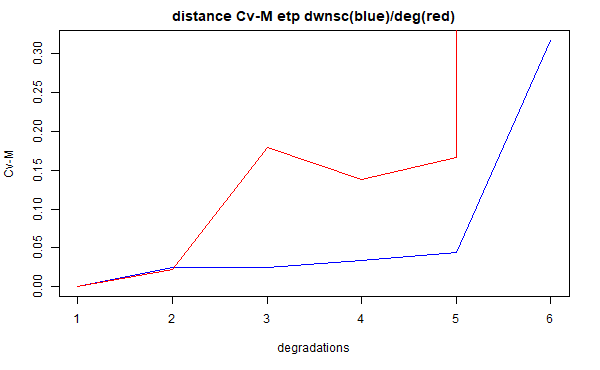
\includegraphics[scale=0.4]{images/Dist_CVM_evap_CDFt.png}
	\end{subfigure}
	\caption{Tracé de la distance de Cramér-von Mises: séries dégradées en rouge et séries downscalées avec l'algorithme CDFt en bleu}
\end{figure}

L'on voit que la projection après downscaling est plus mauvaise  pour les précipitations que seulement la série dégradée pour la distance de Cramer-von Mises, jusqu`à la dégradation $d=3$, et qu'à partir de la dégradation $4$ la série donwscalées est plus proche pour la distance de Cramér-von Mises ($d=5$ sont les données $IPSL$). L'algorithme CDFt est très efficace pour les données IPSL. Il semble que la correction ne soit efficace qu'à partir d'une certaine dégradation ce qui paraît tout de même étonnant. Une explication que nous pouvonss conjecturer est que les erreurs arithmétiques induites par les manipulation informatique des valeurs numériques peut augmenter naturellement ce type d'erreur. Cette explication ne semble pas vraiment convaincante, puisque la courbe devrait quand même suivre la tendance de dégradation et il semble d'après ce graphique que ca ne soit pas le cas.

Cette erreur manifestée par la distance Cramér-von Mises soulève un point que nous n'avons pas encore abordé, c'est le fait que notre échantillon des précipitations possède de nombreuses valeurs à $0$. Cela signifie que la densité n'est plus une fonction mais une distribution avec une dirac en $0$. Nous avons parlé à la fin de la section \ref{ch:CDFt} que les transformations de CDFt gérait mal les variables aléatoire à la fois discrètes et continues.

Regardons maintenant les résultats de l'évaluation de la distance de Cramer-Von Mises pour les séries donscalées par l'algorithme quantile-quantile:

\begin{figure}[H]
 	\label{fig-res_CVM_QQ}
 	\centering
 	\begin{subfigure}[b]{0.45\textwidth}
 		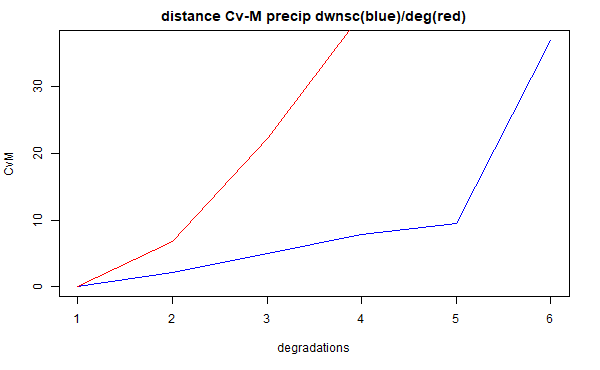
\includegraphics[scale=0.4]{images/Dist_CVM_precip_QQ.png}
 	\end{subfigure}
	\hfill
	\begin{subfigure}[b]{0.45\textwidth}
		\includegraphics[scale=0.4]{images/Dist_CVM_evap_QQ.png}
	\end{subfigure}
 	\caption{Tracé de la distance de Cramér-von Mises: séries dégradées en rouge et séries downscalées avec l'algorithme quantile-quantile en bleu}
\end{figure}

Nous voyons que la distance de Cramér-von Mises s'est considérablement améliorée pour les précipitations, les distances pour l'évapotranspiration sont étonnament proches. Néanmoins regardons les droites de régression quand on affiche les points des séries projetées en fonction des points des séries de référence. 

\begin{figure}[H]
	\begin{minipage}[b]{0.4\linewidth}
		\centering \includegraphics[scale=0.4]{images/pr_3_QQ_ref.png}
	\end{minipage}\hfill
	\begin{minipage}[b]{0.4\linewidth}	
		\centering \includegraphics[scale=0.4]{images/pr_3_dg.png}
	\end{minipage}
	\begin{minipage}[b]{0.4\linewidth}
		\centering \includegraphics[scale=0.4]{images/pr_4_QQ_ref.png}
	\end{minipage}\hfill
	\begin{minipage}[b]{0.4\linewidth}	
		\centering \includegraphics[scale=0.4]{images/pr_4_dg.png}
	\end{minipage}
	\caption{Tracé des précipitations downscalées (quantile-quantile) en fonctions des précipitations de référence pour différentes dégradations PAS LES BONS GRAPHIQUES!!!!!!!!!!!!!!!!!!!!!!!}
\end{figure} 


Les résultats sont ici beaucoup moins bons (si on a les bons graphiques). On choisit finalement les données downscalées par l'algorithme CDFt-SSR.

\subsection{Simulation hydrologique avec HydroGéosphère}

Une fois que l'on a nos données downscalées, il a fallu faire la simulation hydrologique du bassin du Little Washita. Cependant, une modélisation complète du Little Washita ne permettait pas de faire tourner nos modèles dans des délais raisonnables comparés au temps du stage (plus de 2 mois selon l'étudiante avec qui j'ai eu la chance de travailler). Il fallait donc utiliser le modèle simplifié que celle-ci avait développé. Nous commencerons par expliquer ce modèle, puis nous expliquerons les problématiques du spin-up pour l'initialisation des modèles.  

\subsubsection{Modélisation Little Washita HGS}

Une modélisation très rigoureuse du bassin du Little Washita a été faite durant la thèse de \cite{maquin2016developpement}, elle a discrétisé le bassin versant par triangulation (voir figure \ref{fig-Little Washita 3D})

\begin{figure}[H]
	\label{fig-Little Washita 3D}
	\begin{center}
		\includegraphics[scale=0.2]{images/little_washita3D.png}
	\end{center}
	\caption{Maillage tridimensionnel du bassin versant du Little Washita (thèse \cite{maquin2016developpement})}
\end{figure}

L'idée est alors de proposer un modèle beaucoup plus simple permettant de modéliser les écoulements ainsi que les... 

À compléter...




\subsubsection{La problématique du spin-up}

Ici je veux parler de la problématique d'intialisation de la nappe, surtout lorsque le Little Washita souffre d'aridification, donc la nappe diminue chaque an. 

À compléter...

\subsection{Comparaison et analyse des résultats des simulations hydrologiques}

Nous avons donc downscalé nos séries. On a rentré les séries de précipitation et d'évaporation downscalées dans le simulateur d'hydrogéosphère et avons récupérer les séries des débits et des eaux entrantes qui vérifient

\[\textit{eau entrante}=\textit{précipitation}-\textit{évapotranspiration réelle}.\]

Nous allons alors commencer par regarder si la modélisation hydrologique avec downscaling permet de meilleures simulation qu'avec des séries dégradées. Nous analyserons ensuite brièvement la réponse de débits de sorti du modèle en fonction des précipitations entrantes en montrant la non linéarité entre les entrées et les sorties. Finalement, nous verrons qu'il existe des données pour lesquelles les différences des précipitations ont une influence direct sur les différences des débits et nous essaierons d'y trouver une explication.
 
\subsubsection{L'efficacité du downscaling}

Nous allons utiliser les mêmes outils que ceux utilisés dans la partie sur le downscaling pour étudier la qualité de nos simulations, c'est dire qu'on considérera les données des débits obtenus à partir des séries de précipitations et d'évaporation potentielle de référence comme les débits de référence. Et l'on considérera les débits dégradées et évaporation dégradés, ou downscalés, à partir des simulations réalisées avec les données dégradées ou downscalées et nous allons comparer ces séries entre-elles. 


\begin{note}
	Changer l'ordre de grandeur des débits
\end{note}

\vspace{0.7 cm}

\noindent\textbf{Résultats et comparaison conjointe des séries de précipitations et de débits}

\begin{figure}[H]
	\begin{center}
		\includegraphics[scale=0.35]{images/multi_comparaison_2.png}\\
	\end{center}
\caption{Comparaison conjointe des précipitations et des débits pour la dégradation 1}
\end{figure}
\begin{figure}[H]
	\begin{center}
		\includegraphics[scale=0.35]{images/multi_comparaison_3.png}\\
	\end{center}
\caption{Comparaison conjointe des précipitations et des débits pour la dégradation 2}
\end{figure} 
\begin{figure}[H]
	\begin{center}
		\includegraphics[scale=0.35]{images/multi_comparaison_4.png}\\
	\end{center}
\caption{Comparaison conjointe des précipitations et des débits pour la dégradation 3}
\end{figure} 
\begin{figure}[H]
	\begin{center}
		\includegraphics[scale=0.35]{images/multi_comparaison_5.png}\\
	\end{center}
	\caption{Comparaison conjointe des précipitations et des débits pour la dégradation 4}
\end{figure} 

Nous voyons deux choses à partir de ces résultats, la première c'est qu'il y a une forte correspondance entre les droites de régressions pour les séries de précipitation et les série des débits pour une même dégradation. La deuxième c'est que la réponse des débit n'est pas une réponse linéaire. Nous allons essayer de quantifier la non linéarité de cette réponse.
 

\subsubsection{Non linéarité de la réponse débit/précipitation}

Pour étudier la non linéarité des sorties des débit en fonction des entrées des précipitations, on trace la série des débits en fonction de la série des précipitations. On fait alors une régression linéaire à l'ordre 3 pour caractériser la non linéarité de la réponse. Nous ne le ferons que pour la série de référence, mais il est intéressant de voir que la régression linéaire donne parfois un coefficient négatif à l'ordre 3. Ce qui implique que le modèle ne peut pas non-plus être bien approximé par un modèle quadratique.
  
\begin{figure}[H]
	\begin{center}
		\includegraphics[scale=0.45]{images/deb_rapport_pr_deg1.png}\\
	\end{center}
	\caption{Comparaison conjointe des précipitations et des débits pour la dégradation 4}
\end{figure} 

On voit, dans ce cas que la réponse est quadratique (voir exponentielle). On peut faire un rapprochement entre ce résultat et le modèle de Horton. La quantité des écoulements de surface en fonction des précipitations est une réponse exponentielle. 

Peut-être à développer...

\vspace{0.7cm}

\noindent\textbf{Études des lois de distribution pour les séries downscalées et dégradées et distance de Cramér-von Mises}

\begin{figure}[H]
	\label{fig-res_CVM_deb_CDFt}
	\centering
	\begin{subfigure}[b]{0.45\textwidth}
		\includegraphics[scale=0.4]{images/Dist_CVM_CDFt_deb.png}
	\end{subfigure}
	\hfill
	\begin{subfigure}[b]{0.45\textwidth}
		\includegraphics[scale=0.4]{images/Dist_CVM_CDFt_etr.png}
	\end{subfigure}
	\caption{Tracé de la distance de Cramér-von Mises: séries dégradées en rouge et séries downscalées avec l'algorithme quantile-quantile en bleu}
\end{figure}

Étonnamment, les résultats de CDFt se sont inversés pour les débits par rapport aux précipitations et pour l'évaporation réelle par rapport à l'évaporation potentielle (bien que les résultats n'aient pas réellement changés). On remarque que les distances de Cramér-von Mises se sont fortement réduites après passage dans le modèle de simulation hydrologique. Ce résultat est très intéressant, il montre que le filtre de simulation hydrologique contracte les lois de répartitions. 


\subsubsection{Classifications des données réactives et non réactives aux précipitations}
\label{ch:classification delta deb delta pluie}

Nous allons continuer d'étudier l'influence des précipitations sur les résultats de débits. Pour cela, nous étudions séries des différences des débits dégradés ou downscalés et de la série de référence (série observée sur le point du Little Washita) en fonction des séries des différences des précipitations dégradées ou downscalées et de la série des débit simulés à partir des série de précipitation et d'évapotranspiration de référence. Plus formellement, en définissant $(R^{*}_t)_{t \in \llbracket 0, T\rrbracket}$ une série projetée (dégradée ou downscalée) de précipitation et $(R_t)_{t \in \llbracket 0, T\rrbracket}$ la série réelle des précipitations, ainsi que $(Q^{*}_t)_{t \in \llbracket 0, T\rrbracket}$ et $(Q_t)_{t \in \llbracket 0, T\rrbracket}$ une séries de débits projetés et réel. On s'intéresse alors à l'influence de la différence entre les séries projetées $(R^{*}_t)_{t \in \llbracket 0, T\rrbracket}$ et la série réelle de précipitation sur la différence entre les débits projetés et les débits réels. On appelles alors quand c'est défini $\Delta R$ et $\Delta Q$ la différence de la série projetée à la série de référence 
\[\Delta R_t=\frac{R^{*}_t-R_t}{R_t}, \hspace{4mm} \frac{Q^{*}_t-Q_t}{Q_t}.\]
Voici les résultats obtenus pour la série downscalée correspondant à la dégradation $3$:
\begin{figure}[H]
	\label{fig-deb_prec_3}
	\begin{center}
		\includegraphics[scale=0.25]{deb_prec_dec1.png}
	\end{center}
	\caption{Tracé des $\Delta Q_t$ en fonction des $\Delta R_{t+1}$ pour la dégradation $(\times49)$}
\end{figure}

Nous avons en effet affiché les débits du temps $t$ en fonction des précipitation du temps $t+1$, on voit clairement un phénomène corrélation linéaire pour certains débits. Nous cherchons donc à trouver les droites de corrélation (voir section \ref{indexe3:cl_deb}). Après avoir classifié nos points en deux échantillons, la méthode classification est très simple on associe chaque point à sa droite la plus proche. On obtient visuellement cette classification

\begin{figure}[H]
	\label{fig-deb prec 3 classification}
	\begin{center}
		\includegraphics[scale=0.33]{classification_deb_pr.png}
	\end{center}
	\caption{Classification des points selon les droites de régression, dégradation $(\times 49)$}
\end{figure}

On considère maintenant les précipitations réelles entrée dans le sol, HydroGéosphère considère la pluie entrant dans le sol comme étant: 
\[\textit{pluie entrant dans le sol}=\max(\textit{précipitation}-\textit{évapotranspiration},0).\]
On regarde alors la figure des points correspondants pour la pluie entrant dans le sol (on a enlevé toutes le points où la pluie entrant dans le sol était nulle).

\begin{figure}[H]
	\label{fig-deb prr 3 classification}
	\begin{center}
		\includegraphics[scale=0.33]{classification_deb_prr.png}
	\end{center}
	\caption{Classification des points selon les droites de régression pour l'eau entrant dans le sol, dégradation $(\times 49)$}
\end{figure}

Il semble que de nombreux points bleus ont été supprimés. Nous voyons que la classification reste encore effective. L'hypothèse que nous en faisons est que les points bleus correspondent à des temps où la surface de la zone de suintement est faible ou que la cote piezométrique soit grande, alors que les points bleus correspondent à des temps où la surface de la zone de suintement est grande. Nous n'avons malheureusement pas pu vérifier cette hypothèse.

\subsection{Conclusion de l'analyse des données sur le bassin du Little Washita} 

Reste encore à écrire.

\newpage
\section{Annexes}

Ces annexes ont été écrites pour la joie de faire des mathématiques et ne sont en aucun cas nécessaires à la compréhension de ce rapport. Elles ont pour objectif de fournir la plupart des détails mathématiques permettant une compréhension plus complète de certains outils, d'hypothèses ou de méthodes utilisées dans ce mémoire. Il est évident que ce but est loin d'être accompli et qu'il en faudrait beaucoup plus que convenable pour couvrir l'entièreté des sujets abordés dans ce mémoire.
 
\subsection{Annexe 1: Preuves et outils utilisés dans le downscaling}
\label{ch:outils-mathematiques}

\begin{proposition}
	Soit $X$ et $Y$ deux variables aléatoires réelles ayant des fonctions de répartition $\mathcal{F}_{X}$ et $\mathcal{F}_{Y}$ continues, alors 
	$\mathcal{F}^{-1}_Y (\mathcal{F}_X(X))$ et $Y$ suivent la même loi. 
\end{proposition}
\begin{proof}
	Montrons que $\mathcal{F}^{-1}_Y \circ \mathcal{F}_X(X)$ et $Y$ possède la même fonction de densité. 
	\[\mathcal{F}_{\mathcal{F}^{-1}_Y \circ \mathcal{F}_X(X)}(y)
	= \mathbb{P}(\mathcal{F}^{-1}_Y (\mathcal{F}_X(X))\leq y )
	= \mathbb{P}(\mathcal{F}_{X}(X) \leq \mathcal{F}_Y(y)),\]
	comme $\mathcal{F}_{X}(X)$ suit une loi uniforme sur $[0,1]$ si $F_X$ est continue cette égalité se réécrit
	\[= \mathbb{P}(\mathcal{U}(0,1) \leq \mathcal{F}_Y(y))=\mathcal{F}_Y(y).\]
\end{proof}
\begin{proposition}
	\label{mean-rep-emp}
	Soient $X_1,...,X_n,$ $n$ réalisations d'une variable aléatoire réelle $X$ et $\mathcal{F}_{n}$ sa fonction de répartition empirique nous avons
	\[E[\mathcal{F}_n]=F_{X},\]
	alors la fonction de répartition empirique est un estimateur sans biais de la lois de $F$. 
\end{proposition}

\begin{proof}
	C'est en effet évident puisque $\mathds{1}_{[X, +\infty )}(x)$ suit une lois de Bernoulli de paramètre $\mathcal{F}(x)$ alors 
	\[E\Big[\frac{1}{n}\sum_{i=1}^{n}\mathds{1}_{[X_i, +\infty )}(x)\Big]= \frac{1}{n}\sum_{i=1}^{n}E[\mathds{1}_{[X_i, +\infty )}]=\mathcal{F}_{X}(x).\]
\end{proof}


\begin{theorem}(Glivenko-Cantelli)
	\label{th:glivenko}
	Soient $\mathcal{F}_{X}$ et $\mathcal{F}_{n}$ respectivement la fonction de répartition et la fonction de répartition empirique. Alors 
	\begin{equation}
		\|\mathcal{F}_{X}-\mathcal{F}_{n}\|_{\infty} \xrightarrow[n\to \infty]{prob} 0.
	\end{equation}
\end{theorem}

\begin{proof} (Cas où $\mathcal{F}_X$ est continue)
	On commence par remarquer que quelque soit $x$ dans $\mathbb{R}$, \[F_{n}(x)\xrightarrow[n\to \infty]{p.s.}\mathcal{F}_X(x)\] d'après la loi forte des grands nombres et la proposition \eqref{mean-rep-emp}. Pour q dans $\mathbb{Q}$, on définit 
	\[\Omega_{q}=\{\omega \in \Omega | \lim_{n \to \infty} \mathcal{F}_{n}(q)=\mathcal{F}_X(q)\},\]
	d'après ce que nous avons dit, sa mesure pour la probabilité $P(\Omega_q)=1$ comme $\mathbb{Q}$ est dénombrable nous avons  
	\[P\Big(\bigcap_{q \in \mathbb{Q}} \Omega_q \Big)=1.\]
	Alors, comme $\mathbb{Q}$ est dense dans $\mathbb{R}$ et que $\mathcal{F}_{X}$ et les $(\mathcal{F}_n)_{n \in \mathbb{N}}$ sont continues on peut assurer que   
	\[	\|\mathcal{F}_{X}-\mathcal{F}_{n}\|_{\infty} \xrightarrow[n\to \infty]{prob} 0. \]
\end{proof}
Le cas où $\mathcal{F}_{X}$ n'est pas continue est géré par \cite{durrett2019probability} (ex 7.2 chap 1). On voit d'après le théorème \ref{th:glivenko} que la fonction de répartition empirique est le bon estimateur de la fonction de répartition. 


\subsection{Annexe 2: La statistique de Cramér-von Mises}
\label{lemme Cramer-von Mise}
Soient $(X_i)_{i\in \llbracket 1,n \rrbracket}$ et $(Y_i)_{i\in \llbracket 1,m \rrbracket }$ des réalisations indépendante issues des variables aléatoires réelles $X$ et $Y$. On appelle $\mathcal{F}_{n}$ et $\mathcal{G}_{m}$ les fonctions de répartitions empiriques définies à partir de ces réalisation et $\mathcal{H}_{m,n}$ la fonction de répartition empirique définie à partir des réalisations $(Z_i)_{i\in \llbracket 1,m+n \rrbracket }=X_1,...,X_n,Y_1,...,Y_m$. Par la suite on considéra que tous les éléments sont triés dans leur ensemble (c.à.d. $i\leq j \Rightarrow E_i\leq E_j$). Nous avons alors l'égalité suivante
\begin{equation}
	C_{n,m}=\frac{nm}{n+m}\int_{\mathbb{R}}\big[ \mathcal{F}_{n}(x)-\mathcal{G}_{m}(x)\big]^{2} \mathrm{d} \mathcal{H}_{m,n}(x)=\frac{1}{nm(m+n)}\Big[ n\sum_{i=1}^{n}(R_{X_i}-i)^2+ m\sum_{i=1}^{m}(R_{Y_i}-i)^2\Big]-\frac{4nm-1}{6(m+n)}.
\end{equation}
où $R_{Z_i}$ est le rang de $Z_i$ dans $X_1,...,X_n,Y_1,...,Y_n$ autrement dit 
\[R_{X_i}=Card(\{j \in \llbracket 1,m+n \rrbracket , Z_j\leq Z_i\}).\] 
Notons que cette égalité transforme un problème d'analyse en un problème de dénombrement beaucoup plus simple. On rappelle la définition de l'intégrale par rapport à une fonction.
\begin{definition}
	Soient $f:\mathbb{R} \to \mathbb{R}$ et $g:\mathbb{R} \to \mathbb{R}$ deux fonctions continues par morceaux on définit l'intégrale de $f$ par rapport à $g$ comme étant
	\[\int_{\mathbb{R}}f(x)\, dg(x)=lim_{n\to\infty}\sum_{i \in \mathbb{Z}}f(x_{i,n})\big( g\big(x_{i,n}\big)-g\big(x_{i,n-1})\big),\hspace{4mm}x_{i,n}=i/n.\]
\end{definition}

\begin{proof}
	
	\noindent Commencons par montrer l'égalité
	\[\frac{nm}{n+m}\int_{\mathbb{R}}\big[ \mathcal{F}_{n}(x)-\mathcal{G}_{m}(x)\big]^{2} \mathrm{d} \mathcal{H}_{m,n}(x)=\frac{mn}{(m+n)^2}\sum_{i=1}^{m+n}\big(\mathcal{F}_n(Z_i)-\mathcal{G}_{m}(Z_i)\big)^2.\]
	On pose $\delta=\inf \{|Z_i-Z_j|, Z_i \neq Z_j\}$, quel que soit $n\geq n_0$ tel que $1/n_0< \delta$ on a: 
	\[\sum_{i \in \mathbb{Z}}\big(\mathcal{F}_n(\frac{i}{n})-\mathcal{G}_{m}(\frac{i}{n})\big)^2\Big( \mathcal{H}_{m,n}\big(\frac{i}{n}\big)-\mathcal{H}_{m,n}\big(\frac{i-1}{n}\big)\Big)=\sum_{i=1}^{m+n}\big(\mathcal{F}_n(Z_i)-\mathcal{G}_{m}(Z_i)\big)^2,\]
	on obtient donc directement l'égalité voulue en passant à la limite.
	
	Observons maintenant que $\mathcal{F}_n(X_i)=i/n$ et $\mathcal{G}_m(X_i)=(R_{X_i}-i)/m$ ainsi que $\mathcal{F}_n(Y_i)=(R_{Y_i}-i)/n$ et $\mathcal{G}_m(X_i)=i/m$. On peut alors réécrire $C_{n,m}$ en séparant la somme sur les $X_i$ et $Y_i$
	\[C_{n,m} = \frac{mn}{(m+n)^2}\Big[\sum_{i=1}^{n} \Big(\frac{i}{n}-\frac{R_{X_i}-i}{m}\Big)^2+ \sum_{i=1}^{m}\Big(\frac{R_{Y_i}-i}{n}-\frac{i}{m}\Big)^2 \Big]\]
	\[=\frac{mn}{(m+n)^2}\Big[\frac{1}{m^2}\sum_{i=1}^{n}\Big(R_{X_i}-i\frac{m+n}{n}\Big)^2 +
	\frac{1}{n^2}\sum_{i=1}^{m}\Big(R_{Y_i}-i\frac{m+n}{m}\Big)^2\Big]\]
	Remarquons que $C_{n,m}$ est de la forme
	\[C_{n,m}=\frac{mn}{(m+n)^2}\Big[\frac{C_1}{m^2}+\frac{C_2}{n^2} \Big],\]
	et que $C_1$ et $C_2$ sont symétriques en $n$ et $m$. On définit $\Sigma_1=\sum_{i=1}^{n}R^{2}_{X_i}$, $\Sigma_2=\sum_{i=1}^{m}R^{2}_{Y_i}$ et $\mathcal{S}_{k}=\sum_{i=1}^{k}i^2$ nous allons travailler sur l'expression
	\[C_1=\sum_{i=1}^{n}\Big(R_{X_i}-i\frac{m+n}{n}\Big)^2.\]
	On la développe puis factorise pour obtenir
	\[C_1=\frac{m+n}{n}\sum_{i=1}^{n}(R_{X_i}-i)^2-\frac{m}{n}\Sigma_1+\frac{m(m+n)}{n^2}\mathcal{S}_n.\]
	On obtient de la même manière
	\[C_2=\frac{m+n}{m}\sum_{i=1}^{m}(R_{Y_i}-i)^2-\frac{n}{m}\Sigma_2+\frac{n(m+n)}{m^2}\mathcal{S}_m.\]
	D'après ce qu'on a dit précédemment on a donc: 
	\[C_{n,m}=\frac{1}{nm(m+n)}\Big[ n\sum_{i=1}^{n}(R_{X_i}-i)^2+ m\sum_{i=1}^{m}(R_{Y_i}-i)^2\Big]-\frac{\Sigma_1+\Sigma_2}{(m+n)^2}+ \frac{\mathcal{S}_n}{n(n+m)}+ \frac{\mathcal{S}_m}{m(m+n)}.\]
	
	On remarque $\Sigma_1+\Sigma_2 = \mathcal{S}_{m+n}$ et que l'on a la première moitié de notre somme. 
	Il ne reste plus qu'à développer l'expression 
	\[-\frac{\mathcal{S}_{m+n}}{(m+n)^2}+ \frac{\mathcal{S}_n}{n(n+m)}+ \frac{\mathcal{S}_m}{m(m+n)}\]
	\[=-\frac{(m+n+1)(2m+2n+1)}{6(m+n)}+ \frac{(n+1)(2n+1)}{6(m+n)}+\frac{(m+1)(2m+1)}{6(m+n)}=-\frac{4mn-1}{6(m+n)}\]
	En regroupant nos deux résultats nous avons finalement:
	\[C_{n,m}=\frac{1}{nm(m+n)}\Big[ n\sum_{i=1}^{n}(R_{X_i}-i)^2+ m\sum_{i=1}^{m}(R_{Y_i}-i)^2\Big]-\frac{4nm-1}{6(m+n)}\]
\end{proof}	

\subsection{Annexe 3: La projection conique conforme de Lambert}
\label{proj-Lambert}
La plupart des fonctions de projection de $S(\mathbb{R}^3)$ dans $\mathbb{R}^2$ sont des surfaces développables sur lesquelles on projette les points de la terre. Par exemple des cônes, des cylindres et des plans (projection stéréographique) sont les surfaces développable les plus connues. La \textbf{projection Lambert} est une projection conique aussi appelée la projection orthomorphique. Ses caractéristiques sont décrites dans le livre \cite{grafarend2014map}. Elle possède la caractéristique de préserver les angles et les distances pour deux latitudes choisies, pour les données NARR les latitudes choisies sont $33^{\circ}$N et $45^{\circ}$N. De plus les lignes de latitudes égales sont des cercles et celles de longitudes égales des lignes droites. Les coordonnées que nous étudions sont entre $33^{\circ}$N et $36^{\circ}$N. On va montrer que les longueurs étudiées dans cette zone de l'espace ne souffrent que de très peu de déformation. 

\begin{figure}[H]
	\label{fig-proj Lambert}
	\begin{center}
	\includegraphics[scale=0.6]{lambert.jpg}
	\end{center}
\caption{Projection conique conforme de Lambert}
\end{figure}
\begin{definition}
	On définit les fonctions $lat:S(\mathbb{R}^3)\to [-\pi/2,\pi/2] $ et $lon:S(\mathbb{R}^3) \to [-\pi,\pi] $ qui associent à chaque point $x$ de $S(\mathbb{R}^3)$ sa latitude et sa longitude en radiant.
\end{definition} 
\begin{definition}
	On définit le cône convexe $\zeta_{\theta,\theta+\epsilon}$ comme l'ensemble des droites passant les points $x_1$ et $x_2$ de même longitudes de latitudes égale à $\theta$ et $\theta+\epsilon$. Autrement dit
	\[\zeta_{\theta,\theta+\epsilon}=\{D(x_1,x_2), \, x_1,x_2 \in S(\mathbb{R}^3), \, lon(x_1)=lon(x_2),\, lat(x_1)=\theta,\, lat(x2)=\theta+\epsilon\}.\] 
	où $D(x_1,x_2)$ est la droite passant par $x_1$ et $x_2$.
\end{definition}


Il est évident que pour les lignes de latitude haute ($\theta+ \epsilon$) et basse ($\theta$) les longueurs sont conservées. On définit $\epsilon=\pi (45-33)/180$. 


\begin{proposition}
	Pour toute courbe $\gamma: [0,1] \to S(\mathbb{R}^3)$ continue dont les latitudes sont comprises entre $\theta$ et $\theta+\epsilon$, on a 
	\[\min\Big(\cos(\epsilon/2),\frac{\cos(\theta+\epsilon)}{\cos(\theta)} \Big)\leq \frac{\|P(\gamma)\|_{\|\cdot\|_{\mathbb{R}^2}}}{\|\gamma\|_{\|\cdot\|_{S(\mathbb{R}^3)}}} \leq 1.\]
	Où $P$ est la projection de Lambert conservant les longueurs pour les latitudes $\theta$ et $\theta+\epsilon$.
\end{proposition} 
Ce résultat permettra de conclure que la géométrie des lieux peux être considérée comme euclidienne si $\epsilon$ est suffisamment petit.

\begin{proof} (Esquisse) On montrera cette inégalité pour les courbes de latitudes constantes et pour celles de longitudes constantes et la densité des fonctions de longitude ou de latitude par morceaux constantes dans l'ensemble des courbes permettra de conclure cette inégalité pour toutes les courbes.
	
\vspace{4mm}
	
On définit trois ensembles de courbes, $\mathcal{C}_1$, $\mathcal{C}_2$ et $\mathcal{C}_{m}$ tels que \[\mathcal{C}_1=\{\gamma \in \mathcal{C},\, lon(\gamma(t))=c, \, \forall t \in [0,1],\]
\[\mathcal{C}_2=\{\gamma \in \mathcal{C},\, lat(\gamma(t))=c, \, \forall t \in [0,1]\},\]
\[\mathcal{C}_m=\{\gamma \in \mathcal{C},\, \exists t_1<...<t_n,\forall \leq i<n, \gamma_i: t \mapsto \gamma(t_i+ t(t_{i+1}-t_i)) \in \mathcal{C}_1 \cup \mathcal{C}_2\}.\]
On commence par étudier les courbes $\gamma$ dans $\mathcal{C}_1$ injectives, on peut alors sans perte de généralité se placer dans le cas du cercle unité dans $\mathbb{R}^2$ (le cercle de longitude constante). On a alors l'égalité
	
\[\|\gamma\|_{\|\cdot\|_{S(\mathbb{R}^3)}}=\|\gamma\|_{\|\cdot\|_{S(\mathbb{R}^2)}}=\int_{0}^{1}|\gamma'(t)|dt.\]
\begin{figure}[H]
	\label{fig-Lambert schema exp }
	\begin{center}
		\includegraphics[scale=0.25]{geogebra_lambert.png}
	\end{center}
	\caption{Figure explicative de la projection conique conforme de Lambert}
\end{figure}
	
D'après ce schéma, on voit que pour tout point $F$ sur le cercle la longueur de la courbe $\gamma$ allant de $B$ à $F$  est majorée par la longueur du segment $BI$, de plus sur la figure  on a $\epsilon/2=\beta$. On obtient facilement l'inégalité
\[\cos(\epsilon/2)\leq\frac{\|P(\gamma)\|_{\|\cdot\|_{\mathbb{R}^2}}}{\|\gamma\|_{\|\cdot\|_{S(\mathbb{R}^3)}}}.\]
	
Étudions maintenant les courbes $\gamma$ dans $\mathcal{C}_2$ de latitude égale à $\theta+\epsilon$ et injectives. On sait que la courbe $\gamma$ ainsi que sa projection $P(\gamma)$ décrivent un arcs de cercle dans $\mathbb{R}^3$. Le rapport entre la longueur de l'arc de cercle définit par $P(\gamma)$ et $\gamma$ dans $\mathbb{R}^3$ est majoré grossièrement par $\cos(\theta+\epsilon)/\cos(\beta)$. Alors, quelque soit $\gamma$ dans $\mathcal{C}_2$ on
\[\frac{\cos(\theta+\epsilon)}{\cos(\beta)}\leq\frac{\|P(\gamma)\|_{\|\cdot\|_{\mathbb{R}^2}}}{\|\gamma\|_{\|\cdot\|_{S(\mathbb{R}^3)}}}\]
Pour chaque courbe $\gamma$ dans $\mathcal{C}_m$ on a alors 
\[\min\Big(\frac{2\sin(\epsilon/2)}{\epsilon},\frac{\cos(\theta+\epsilon)}{\cos(\theta)} \Big)\leq \frac{\|P(\gamma)\|_{\|\cdot\|_{\mathbb{R}^2}}}{\|\gamma\|_{\|\cdot\|_{S(\mathbb{R}^3)}}} \leq 1,\]
la densité de $\mathcal{C}_m$ dans l'ensemble des courbes continues permet de conclure.
\end{proof}

Finalement, on peut voir que dans notre cas où $\theta=\pi 33/180$ et $\epsilon=\pi 12/180$. On a que pour toute courbe $\gamma:[0,1]\to S(\mathbb{R}^3)$ dont la latitude est comprise entre $\theta$ et $\theta+\epsilon$ on a
\[0.84\leq \frac{\|P(\gamma)\|_{\|\cdot\|_{\mathbb{R}^2}}}{\|\gamma\|_{\|\cdot\|_{S(\mathbb{R}^3)}}} \leq 1.\]


\subsection{Annexe 4: Classification des populations de débit}
\label{indexe3:cl_deb}

On commence par rappeler ce que sont les données $\Delta Q$ et $\Delta R$, sont les différences entre les séries projetées et les séries de référence ($R$ correspond à la pluie et $Q$ au débit). Nous avons vu  que les schémas nous incitent à considérer deux classes de points (citer la partie correspondante).
\begin{figure}[H]
	\label{fig-deb delta Q delta R }
	\begin{center}
		\includegraphics[scale=0.28]{deb_prec_dec1.png}
	\end{center}
	\caption{Tracé des $\Delta Q(t)$ en fonction des $\Delta R(t-1)$}
\end{figure}

On définit alors les ensembles $\mathcal{C}$ et $\mathcal{I}$ tels que
\[\mathcal{C}=\{(\Delta Q(t),\Delta R(t-1)), \, \Delta Q(t)= f(\Delta R(t-1))+\epsilon(t)\},\]
où $\epsilon$ est un bruit blanc et $f$ une fonction affine, et
\[\mathcal{I}= \{(\Delta Q(t),\Delta R(t-1)), \, cov(\Delta Q(t),\Delta R(t-1))=0\},\]
c'est à dire les lorsque les points $\Delta Q(t)$ et $\Delta R(t-1)$ sont indépendants.  

Il parait alors pertinent d'utiliser deux droites $D_1$ et $D_2$ pour classifier ces débits. Et l'on va chercher à définir les ensembles $\mathcal{C}$ et $\mathcal{I}$ à partir de ces deux droites.
Soit $X$ un ensemble de points  $x_1, x_2, .., x_n \in \mathbb{R}^2$, on cherche deux droites $D_1$ et $D_2$ minimisant la valeur
\[\sum_{i=1}^{n}d(x_i, D_1 \cup D_2),\]

où $d$ est la distance définie par 
\[d(x,E)= \min_{e \in E} |x-e|^2.\]
On peut définir les droites de $\mathbb{R}^2$ par un coupe de points $(u,v)$ dans $\mathcal{U}_1(\mathbb{R}^2)\times\mathbb{R}^2$, où $\mathcal{U}_1(\mathbb{R}^2)$ est le cercle unité et $u$ définit la direction de la droite et $v$ sont orientation. Alors, on peut redéfinir le problème dans ce cadre. On cherche les couples $(u_1,v_1)$ et $u_2,v_2$ minimisant la fonction $F$ satisfaisant 
\begin{equation}
	\label{F}
	\begin{array}{cccc}
		F: & (\mathcal{U}_1(\mathbb{R}^2)\times\mathbb{R}^2)^2 &\to &\mathbb{R}\\
		& ((u_1,v_1), (u_2,v_2)) & \mapsto & \sum_{i=1}^{n}\min (d(x_i,\mathbb{R}u_1+v_1), d(x_i,\mathbb{R}u_2+v_2))
	\end{array}
\end{equation}


On commence par développer la distance d'un point à une droite, c'est une formule de projection classique. On appelle $f$ la fonction $f:(\mathcal{U}_1(\mathbb{R}^2)\times\mathbb{R}^2) \times \mathbb{R}^2 \to \mathbb{R}$, $f((u,v),x)=d(x,\mathbb{R}u+v)$.
\begin{equation}
	\begin{array}{ccc}
		f_x(u,v)&=&d(x,\mathbb{R}u+v)\\
		&=& \big|x-v-u\big<x-v , u\big> \big|^2\\
		&=& \big|x-v\big|^2 -\big<x-v, u\big>^2\\
		&=& \big|x\big|^2-2\big<x,v\big>+\big|v\big|^2 -\big<x, u\big>^2+ 2\big<x, u\big>\big<v, u\big>- \big<v, u\big>^2.
	\end{array}
\end{equation}

On cherche maintenant à calculer $\overrightarrow{\nabla} f_x$, le gradient étant une application linéaire, on a  
\[\overrightarrow{\nabla} f_x (u,v)= \overrightarrow{\nabla}\big|x\big|^2-\overrightarrow{\nabla}2\big<x,v\big>+\overrightarrow{\nabla}\big|v\big|^2 -\overrightarrow{\nabla}\big<x, u\big>^2+ \overrightarrow{\nabla}2\big<x, u\big>\big<v, u\big>- \overrightarrow{\nabla}\big<v, u\big>^2,\]
après avoir développé puis factoriser on obtient finalement, 
\begin{equation}
	\overrightarrow{\nabla} f_x (u,v)=2
	\begin{pmatrix}
		(v-x)\big<u,x-v\big>\\
		v-x+u\big<u,x-v\big>
	\end{pmatrix}.
\end{equation}
On peut donc en déduire une formule pour la fonction $F$ définie dans \eqref{F}
\begin{equation}
	\begin{array}{ccc}
		F((u_1,v_1), (u_2,v_2))&=& \sum_{i=1}^{n}\min (f_{x_i}(u_1,v_1) ,f_{x_i}(u_2,v_2) )\\
		&=& \sum_{i=1}^{n} \frac{f_{x_i}(u_1,v_1)+f_{x_i}(u_2,v_2) -\big|f_{x_i}(u_1,v_1)- f_{x_i}(u_2,v_2) \big| }{2}.
	\end{array}
\end{equation}
On obtient finalement une expression pour $\overrightarrow{\nabla} F$, 
\begin{equation}
	\overrightarrow{\nabla} F(u_1,v_1, u_2,v_2)=
	\begin{pmatrix}
		\sum_{i=1}^{n}\mathcal{I^{-}}_{x_i}((u_1,v_1),(u_2,v_2))\overrightarrow{\nabla}f_{x_i} (u_1,v_1)\\
		\sum_{i=1}^{n}\mathcal{I^{+}}_{x_i}((u_1,v_1),(u_2,v_2))\overrightarrow{\nabla}f_{x_i} (u_2,v_2)
	\end{pmatrix}
\end{equation}
où \[\mathcal{I^{-}}_{x_i}((u_1,v_1),(u_2,v_2))=\mathds{1}_{]-\infty,0]}(f_{x_i}(u_1,v_1)- f_{x_i}(u_2,v_2))\] et \[\mathcal{I^{+}}_{x_i}((u_1,v_1),(u_2,v_2))=\mathds{1}_{[0,\infty[}(f_{x_i}(u_1,v_1)- f_{x_i}(u_2,v_2)).\]

On peut appliquer l'algorithme d'Uzawa (voir par exemple \cite{boyd2004convex}) pour trouver le minimum sur  $(\mathcal{U}_1(\mathbb{R}^2)\times\mathbb{R}^2)^2$ en considérant le plongement de $F$ dans  $(\mathbb{R}^2\times\mathbb{R}^2)^2$ avec les contraintes $|u_i|=1$. Nous avons chercher ces droites avec la fonction de minimize de ``scipy.optimize'' voir \cite{scipy}. Les deux droites trouvées sont alors 

\begin{figure}[H]
	\label{fig-deb delta Q delta R avec droites}
	\begin{center}
		\includegraphics[scale=0.28]{deb_prec_dec1_droites.png}
	\end{center}
	\caption{Tracé des $\Delta Q(t)$ en fonction des $\Delta R(t-1)$ avec droites de classification}
\end{figure}

Nous verrons qu'on peut alors classifier les points en deux groupes dont nous essayons de donner une interprétation physique dans la section \ref{ch:classification delta deb delta pluie}.  


\newpage
\bibliographystyle{apalike} 
\bibliography{mabib}

\end{document}